\chapter{Data preprocessing}
\label{chap:data_preprocessing}


\section{Preprocessing Rationale and Technical Constraints}
\label{sec:preprocessing_rationale}

DNA methylation arrays superimpose biological variability and platform-specific
artefacts on the same high-dimensional signal. The exploratory analyses of
Chapter~\ref{sec:data_preparation_exploration} showed that Normal and Adjacent
tissues exhibit nearly identical global distributions, variance profiles, and
correlation structure across all three cohorts. Meaningful differences emerge
exclusively at focal CpG loci — as quantified by locus-specific $\Delta\beta$
distributions and outlier burden ratios — and remain subtle even at that scale
(mean $|\Delta\beta|$ from 0.009 in GSE69914 to 0.031 in GSE287331). This makes
the Normal--Adjacent signal particularly vulnerable to technical confounders
operating at a comparable or larger scale, so preprocessing must be precise:
aggressive enough to remove noise, yet conservative enough to preserve the
epigenetic drift that motivates this thesis.
Three main classes of technical issues must be addressed before any statistical
modelling. First, \emph{probe-design bias} arises from the coexistence of
Type~I and Type~II probes, which produce inherently different $\beta$-value
distributions and distort cross-sample comparability if uncorrected
\cite{Triche2013Noob, Fortin2017}. This issue is not uniform across datasets:
GSE69914 and GSE225845 were released with normalization already applied, whereas
GSE287331 shows clear diagnostic evidence of missing probe-type correction,
requiring an additional decision with non-trivial consequences for downstream
group separation (Section~\ref{sec:dataset_specific}). Second,
\emph{unreliable or biologically confounded probes} — including cross-reactive
loci, SNP-affected sites, non-CpG targets, and sex-chromosome probes — introduce
systematic measurement error that can generate spurious associations or mask
genuine methylation differences \cite{WilhelmBenartzi2013, Xu2021}. Third, the
\emph{statistical scale of $\beta$-values}, with their bounded $[0,1]$ support
and mean-dependent heteroscedasticity, violates the assumptions of standard
parametric models, motivating transformation to a more statistically
well-behaved representation \cite{Triche2013Noob}.

This chapter addresses these issues through a structured, platform-aware pipeline
applied consistently across all cohorts. Section~\ref{sec:pipeline} describes
the general framework; Section~\ref{sec:dataset_specific} documents
dataset-specific decisions, focusing on the handling of probe-type bias in
GSE287331; Section~\ref{sec:inter_preprocessing} summarises the effect of
preprocessing on CpG dimensionality and cross-dataset overlap, providing the
basis for Chapter~\ref{chap:feature_selection}.

\section{General Preprocessing Framework}
\label{sec:pipeline}

This section describes the general preprocessing framework applied to all 
three methylation datasets. The pipeline comprises four sequential steps, 
each addressing a distinct class of technical issue identified in the 
overview above. Two of these steps—data integrity verification and 
Infinium probe-design bias correction—require dataset-specific decisions 
whose rationale and consequences are discussed in 
Section~\ref{sec:dataset_specific}. The remaining two steps—technical 
probe filtering and $\beta$-to-$M$ transformation—are applied uniformly 
across all cohorts following the same protocol.

%------------------------------------------------------------------
\subsection{Structural Integrity and Cohort Harmonization}
\label{subsec:step0}
%------------------------------------------------------------------

Prior to any preprocessing operation, each dataset undergoes a structural 
verification stage to ensure the consistency and completeness of the input 
data. This step checks for correct alignment between the methylation matrix 
and its associated phenotype table, verifies sample identifier uniqueness, 
and confirms the absence of missing metadata fields. Only samples for which 
both a complete methylation profile and a valid tissue label are available 
are retained for downstream analysis.
Probe-level and sample-level missingness in the $\beta$-value matrix is 
also assessed at this stage. For two of the three datasets (GSE69914 and 
GSE225845), the released matrices are fully observed and require no 
imputation. For GSE287331, a non-negligible fraction of CpG sites exhibits 
missing values across samples, necessitating a dedicated filtering and 
imputation strategy consistent with current recommendations for 
EPIC-array quality control~\cite{islam2019_pediatric_dnamm, mansell2019guidance}. The 
dataset-specific treatment of missingness is detailed in 
Section~\ref{subsec:gse287331_data_prep}.

Finally, cohort harmonization is applied where necessary to align tissue 
labels to the three-class framework (Normal, Adjacent, Tumor) adopted 
uniformly across datasets. Samples belonging to tissue categories outside 
this framework are excluded at this stage to ensure cross-dataset 
comparability.

%------------------------------------------------------------------
\subsection{Probe-Type Bias Diagnostics and Correction}
\label{subsec:step1}
%------------------------------------------------------------------

A well-documented source of systematic bias in Illumina Infinium 
methylation arrays is the coexistence of two chemically distinct probe 
designs. Type~I probes use two bead types per CpG (one for the methylated 
channel, one for the unmethylated channel), whereas Type~II probes use a 
single bead type and rely on single-base extension with two-color 
detection. This design difference produces inherently distinct 
$\beta$-value distributions for the two probe types: Type~I probes tend 
to yield more extreme values near 0 and 1, while Type~II probes exhibit 
a broader, intermediate distribution. If uncorrected, this imbalance 
propagates into downstream statistical analyses and can generate 
probe-type-specific artefacts in differential methylation 
testing~\cite{Teschendorff2013BMIQ, maksimovic2012}.
The canonical approach to mitigating this bias is Beta-Mixture Quantile 
normalisation (BMIQ), introduced by Teschendorff et 
al.~\cite{Teschendorff2013BMIQ}. BMIQ explicitly models probe-type bias 
at the $\beta$-value level through a state-aware distributional alignment 
procedure. For each sample independently, a three-component Beta mixture model is 
first fitted to the $\beta$-value distribution of Type~I probes, 
representing unmethylated, partially methylated, and fully methylated 
states. These fitted components define the reference state-specific 
distributions. Type~II probes are then probabilistically assigned to one 
of the three methylation states based on their $\beta$-values, and within 
each state a quantile-mapping step is applied to align the Type~II 
distribution to the corresponding Type~I reference distribution. Because the procedure is performed independently for each sample, BMIQ 
does not introduce cross-sample information or global harmonisation across 
tissue classes; it strictly corrects within-sample probe-type bias.
For each dataset, a systematic diagnostic is performed prior to any 
correction step~\cite{Teschendorff2013BMIQ, Wang2015Normalization450K}: probes are 
stratified by design type using the official Illumina manifest, and two 
complementary assessments are carried out—(i) a density comparison of 
$\beta$-value distributions for Type~I and Type~II probes, and (ii) a 
quantile--quantile plot of Type~II versus Type~I quantiles, with the 
median absolute deviation (MAD) of the empirical Q--Q curve from the identity line 
as a scalar diagnostic metric. Datasets for which the original authors 
applied BMIQ or an equivalent normalisation are expected to exhibit 
near-overlapping distributions and a MAD close to zero; datasets lacking 
probe-type correction will display a pronounced distributional mismatch 
and elevated MAD.

The outcome of this diagnostic, and the corrective action taken, differs 
across cohorts and is reported in full in Section~\ref{sec:dataset_specific}. 
Critically, the decision of whether to apply BMIQ is not made 
mechanically: as discussed in Section~\ref{subsec:gse287331_data_prep}, BMIQ 
correction can attenuate genuine biological structure when group-level 
differences are expressed as broad distributional shifts, a phenomenon 
documented in systematic evaluations of EPIC-array normalisation 
methods~\cite{Yousefi2013, Welsh2023EPICnorm, Liu2016Processing}. The choice between 
correcting and preserving the raw data is therefore made on the basis of 
empirical evidence from the diagnostic plots and quantitative assessment 
of group separability before and after correction.

%------------------------------------------------------------------
\subsection{Technical Probe Filtering}
\label{subsec:step2}
%------------------------------------------------------------------

After addressing probe-design bias, unreliable CpG loci are removed 
through a systematic filtering procedure based on curated external 
annotation resources. The objective is to exclude probes whose measured 
$\beta$-values may reflect technical measurement error rather than 
genuine DNA methylation, thereby reducing noise and improving the 
reliability of downstream differential analyses. Four categories of technically problematic probes are systematically excluded.

\paragraph{Cross-reactive and multi-mapping probes.} Probes that 
hybridise to multiple genomic loci produce $\beta$-values that cannot 
be unambiguously attributed to a single CpG site. These are identified 
using the catalogues of Naeem et al.~\cite{naeem2014}, Chen et 
al.~\cite{chen2013}, Pidsley et al.~\cite{Pidsley2016}, Zhou et 
al.~\cite{zhou2016}, and McCartney et al.~\cite{mccartney2016}. Full 
descriptions of each resource are provided in Appendix~\ref{sec:probe-filters}.

\paragraph{SNP-affected probes.} Probes whose interrogated CpG 
dinucleotide, single-base extension site, or probe body overlaps a 
common genetic variant may measure genotype rather than methylation 
status, producing population-stratified artefacts in group 
comparisons~\cite{zhou2016, Pidsley2016}. These are excluded using the 
\texttt{MASK\_snp5} and \texttt{MASK\_extBase} fields from the Zhou 
annotation~\cite{zhou2016}, supplemented by variant-aware lists from 
Naeem et al.~\cite{naeem2014}.

\paragraph{Non-CpG probes.} Probes targeting non-CpG cytosine contexts 
(identified by the \texttt{ch} prefix in Illumina probe identifiers) are 
excluded, as their interpretation differs from canonical CpG methylation 
and is outside the scope of this analysis~\cite{zhou2016, Pidsley2016}.

\paragraph{Sex-chromosome probes.} Probes located on chromosomes X and Y 
are removed to prevent sex-driven confounding effects. Sex-chromosome 
CpGs exhibit substantially different methylation profiles between males 
and females, and including them in joint normalisation has been shown to 
introduce artificial sex-related bias into autosomal 
probes~\cite{Wang2022InterpolatedXY}. Since the datasets analysed here contain samples 
from both sexes and sex-specific methylation is not the object of 
investigation, removal therefore represents a conservative strategy to prevent confounding without compromising autosomal inference~\cite{maksimovic2012}.

The filtering resources are applied under a union criterion: a probe is removed if it appears in at least one curated list. Platform-specific 
manifests (HumanMethylation450 v1.2 for GSE69914~\cite{Illumina450kAnno}; 
MethylationEPIC v1.0 B5 for GSE225845 and GSE287331~\cite{IlluminaEPIC}) 
are used for manifest-based validation, chromosome annotation, and 
non-CpG probe identification. The number of probes flagged by each 
resource, and the redundancy of flags across resources, are reported 
per-dataset in Section~\ref{sec:dataset_specific}.

%------------------------------------------------------------------
\subsection{Statistical Transformation: $\beta$-to-$M$ Values}
\label{subsec:step3}
%------------------------------------------------------------------

The final preprocessing step transforms the filtered $\beta$-value matrix 
into $M$-values prior to statistical modelling. As defined in Equation~\eqref{eq:beta_definition}, $\beta$-values are bounded proportions in $[0,1]$ derived from methylated and unmethylated probe intensities. While $\beta$-values are intuitive and directly 
interpretable as fractional methylation, their bounded support induces 
strong mean-dependent heteroscedasticity: variance is inflated near 
intermediate values ($\beta \approx 0.5$) and compressed near the 
boundaries, violating the homoscedasticity assumptions underlying 
standard linear modelling frameworks~\cite{Du2010}. The logit transformation to $M$-values,
\begin{equation}
    M = \log_2\!\left(\frac{\beta + \varepsilon}{1 - \beta + \varepsilon}\right),
    \quad \varepsilon = 10^{-6},
    \label{eq:mvalue}
\end{equation}
maps $\beta \in (0,1)$ to an unbounded real-valued scale and 
substantially stabilises the mean--variance relationship~\cite{Du2010}. 
As shown in their analysis, the relationship between $\beta$ and $M$-values 
is a logit transformation yielding an approximately linear correspondence 
in the intermediate methylation range and nonlinear compression at the 
extremes. The small offset $\varepsilon$ is introduced to handle boundary values 
numerically. The resulting $M$-value distributions are approximately 
symmetric and exhibit markedly flatter variance profiles across the full 
methylation range, making them the standard input for differential methylation analysis within linear modelling frameworks and related inferential procedures~\cite{Triche2013Noob, Fortin2017, Thienpont2016}.

It is important to note that $M$-values are adopted exclusively for 
statistical modelling: $\beta$-values are retained in parallel for 
biological interpretation, effect-size quantification, and visualisation, 
following the dual-representation convention recommended by Du et 
al.~\cite{Du2010} and widely adopted in the 
literature~\cite{Thienpont2016, Reinius2012}. 
The transformation is applied to the complete post-filtering matrix for 
each dataset. Distributional diagnostics confirming the expected 
variance-stabilising effect are reported in 
Section~\ref{sec:dataset_specific}. This choice is consistent with the feature-selection and modelling procedures developed in the subsequent Chapter~\ref{chap:feature_selection}, which rely on variance-based ranking, linear statistics, and stability criteria that assume approximately homoscedastic behaviour.

\section{Dataset-Specific Implementation}
\label{sec:dataset_specific}

This section documents the dataset-specific application of the preprocessing pipeline described in Section~\ref{sec:pipeline}. For each cohort, the outcome of structural verification, probe-type bias diagnostics, technical probe filtering, and $\beta$-to-$M$ transformation is reported in detail. Although the general framework is applied consistently across all datasets, certain steps—most notably probe-type bias correction and handling of missing values—require cohort-specific decisions. These are explicitly justified within each subsection.
The results are presented separately for GSE69914 (Section~\ref{subsec:gse69914_preproc}), GSE225845 (Section~\ref{subsec:gse225845_preproc}), and GSE287331 (Section~\ref{subsec:gse287331_data_prep}).


% ============================================================
\subsection{Dataset GSE69914}
\label{subsec:gse69914_preproc}
% ============================================================
\begin{figure}[t]
    \centering
    \begin{subfigure}[t]{0.48\linewidth}
        \centering
        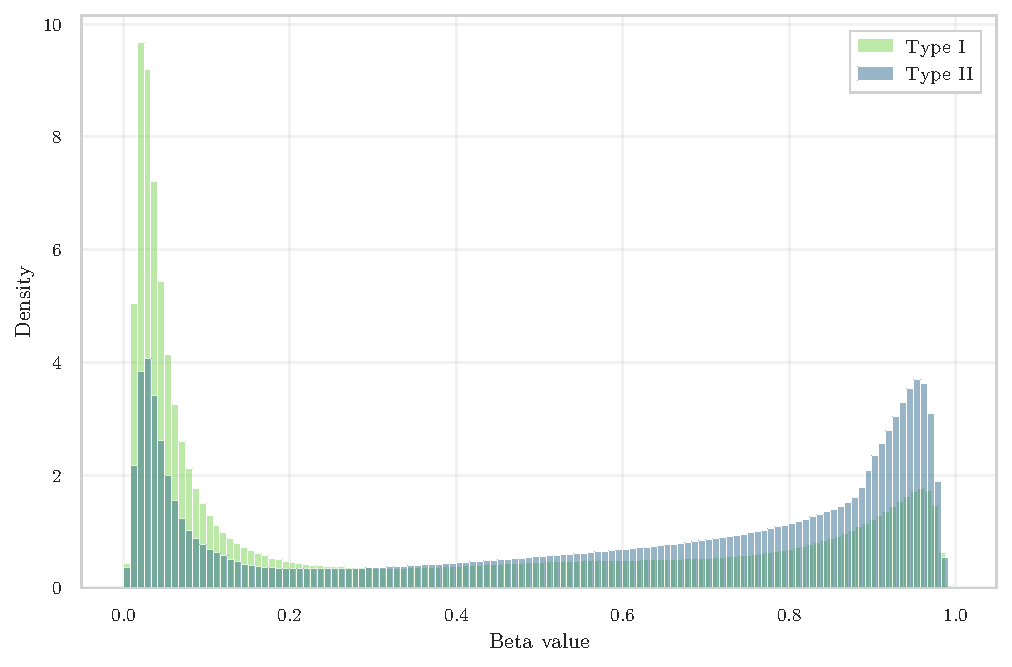
\includegraphics[height=4.5cm,keepaspectratio]{images/cap4/GSE69914_type_bias_density.pdf}
        \caption{$\beta$-value density by probe type.}
        \label{fig:type_bias_density}
    \end{subfigure}
    \hfill
    \begin{subfigure}[t]{0.48\linewidth}
        \centering
        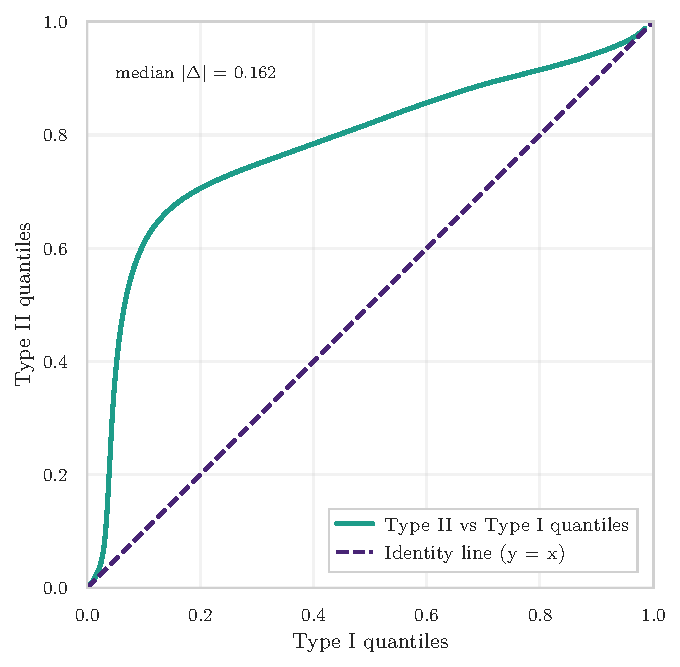
\includegraphics[height=4.5cm,keepaspectratio]{images/cap4/GSE69914_type_bias_qqplot.pdf}
        \caption{Q--Q plot (Type~II vs.~Type~I).}
        \label{fig:type_bias_qq}
    \end{subfigure}
    \caption{Infinium Type~I/II bias diagnostics in GSE69914.}
    \label{fig:type_bias_combined}
\end{figure}

\paragraph{Structural Integrity and Cohort Harmonization}
\label{par:gse69914_step0}
The dataset comprises 397 samples and 485{,}512 CpGs at load time. All sample identifiers are unique, and the phenotype table contains complete metadata for the required fields.
Alignment between the phenotype annotation and the $\beta$-value matrix is exact. The methylation matrix is fully observed, with no missing CpG values and no incomplete samples. No exclusion or imputation was required.

\paragraph{Probe-Type Bias Diagnostics and Correction}
\label{par:gse69914_typebias}

Raw intensity data were reported to have been processed by the original authors using the \texttt{minfi} pipeline with BMIQ normalization~\cite{GSE69914}. Diagnostic evaluation confirms that probe-type bias is effectively mitigated in the released matrix.
The $\beta$-value density distributions of Type~I and Type~II probes exhibit substantial overlap, with no evidence of the characteristic multi-modal distortion observed in uncorrected data (Figure~\ref{fig:type_bias_density}). Quantile--quantile analysis further supports this result: the Type~II versus Type~I quantiles align closely to the identity line, with median absolute deviation $\mathrm{median}|\Delta| = 0.162$, indicating balanced probe-type scaling (Figure~\ref{fig:type_bias_qq}).
Together, these diagnostics are consistent with effective BMIQ correction, in agreement with the normalization behaviour described in~\cite{Teschendorff2013BMIQ, maksimovic2012, Wang2015Normalization450K}.

\paragraph{Technical Probe Filtering}
\label{par:gse69914_step2}

\begin{figure}[t]
    \centering

    % Panel (a)
    \begin{subfigure}[t]{0.48\linewidth}
        \centering
        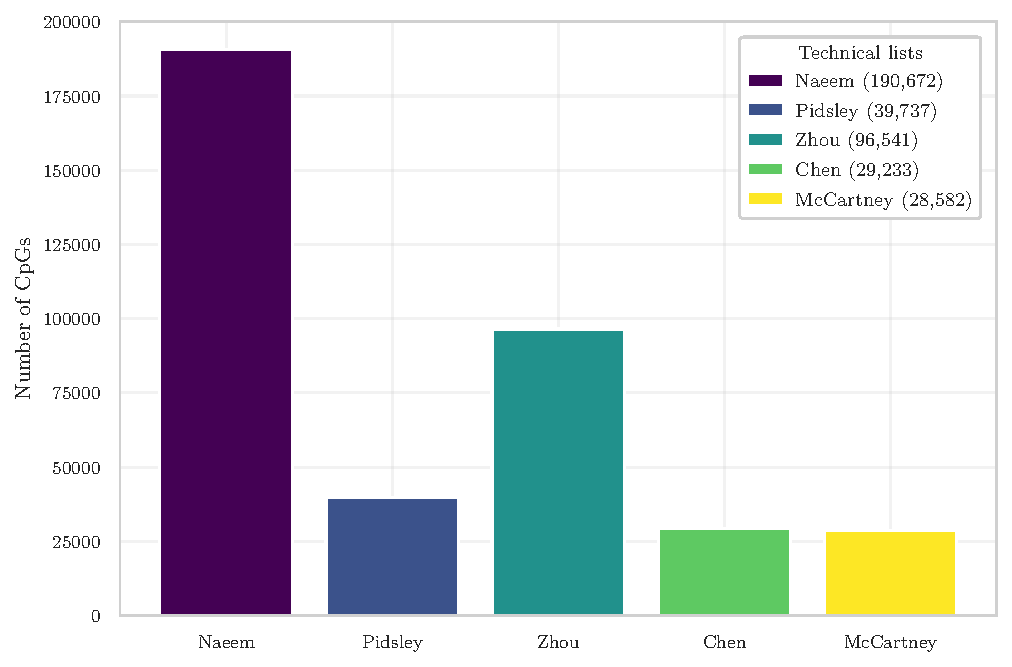
\includegraphics[width=\linewidth]{images/cap4/GSE69914_technical_lists_barplot.pdf}
        \caption{
            CpGs flagged by each technical list. 
        }
        \label{fig:gse69914_tech_barplot}
    \end{subfigure}
    \hfill
    % Panel (b)
    \begin{subfigure}[t]{0.48\linewidth}
        \centering
        \includegraphics[width=\linewidth]{images/cap4/GSE69914_technical_lists_redundancy_histogram.pdf}
        \caption{Redundancy across filtering lists.}
        \label{fig:gse69914_tech_redundancy}
    \end{subfigure}

    \caption{Technical filtering summary in GSE69914.}
    \label{fig:gse69914_technical_filtering}
\end{figure}

\begin{table}[t]
\centering
\caption{CpG filtering summary for the GSE69914 dataset.}
\label{tab:gse69914_cpg_filtering}
\scriptsize
\begin{tabular}{c c c c c c c c c}
\toprule
Initial CpGs &
Naeem &
Pidsley &
Zhou &
Chen &
McCartney &
Non-CpG &
X/Y &
Final CpGs \\
\midrule
485{,}512 &
190{,}672 &
39{,}737 &
96{,}541 &
29{,}233 &
28{,}582 &
875 &
7{,}728 &
251{,}483 \\
\bottomrule
\end{tabular}
\end{table}

Intersection with external technical filtering resources resulted in substantial probe removal, as summarised in Table~\ref{tab:gse69914_cpg_filtering}. The largest individual contributions derive from the Naeem and Zhou annotations, while the remaining resources flag smaller but non-negligible subsets. The redundancy structure across lists is shown in Figure~\ref{fig:gse69914_tech_redundancy}.
Because these catalogues target partially distinct classes of technical artefacts—such as cross-reactivity, SNP interference, and repeat-associated probes—limited overlap across lists is expected. Most excluded CpGs are supported by a single resource, with progressively fewer loci flagged by multiple independent annotations. This pattern reflects complementary rather than redundant filtering criteria, while the subset of probes flagged by several lists indicates concordance for loci exhibiting multiple technical vulnerabilities.
Annotation-based validation using the HumanMethylation450 v1.2 manifest~\cite{Illumina450kManifest} further excluded non-CpG probes and loci lacking reliable genomic annotation. Subsequent removal of sex-chromosome probes (X/Y), consistent with established  preprocessing recommendations in mixed-sex cohorts~\cite{maksimovic2012, Wang2022InterpolatedXY}, ensured a strictly autosomal working set.
A detailed per-probe exclusion summary is available in the project repository at  
\href{https://github.com/elisabettaroviera/THESIS/blob/main/05%20-%20CpG%20list/Removed%20CpGs%20per%20Dataset/removed_cpgs_all_filters_summary_gse69914.csv}
{\texttt{removed\_cpgs\_all\_filters\_summary\_gse69914.csv}}.


\paragraph{Statistical Transformation: $\beta$-to-$M$ Values}
\label{par:gse69914_step4}

% ============================================================
% FIGURES: HISTOGRAMS + MEAN–SD FOR BETA AND M
% ============================================================
\begin{figure}[t]
    \centering

    % ---------------- ROW 1: HISTOGRAMS (Beta, Normal & Adjacent) ----------------
    \begin{subfigure}{0.24\textwidth}
        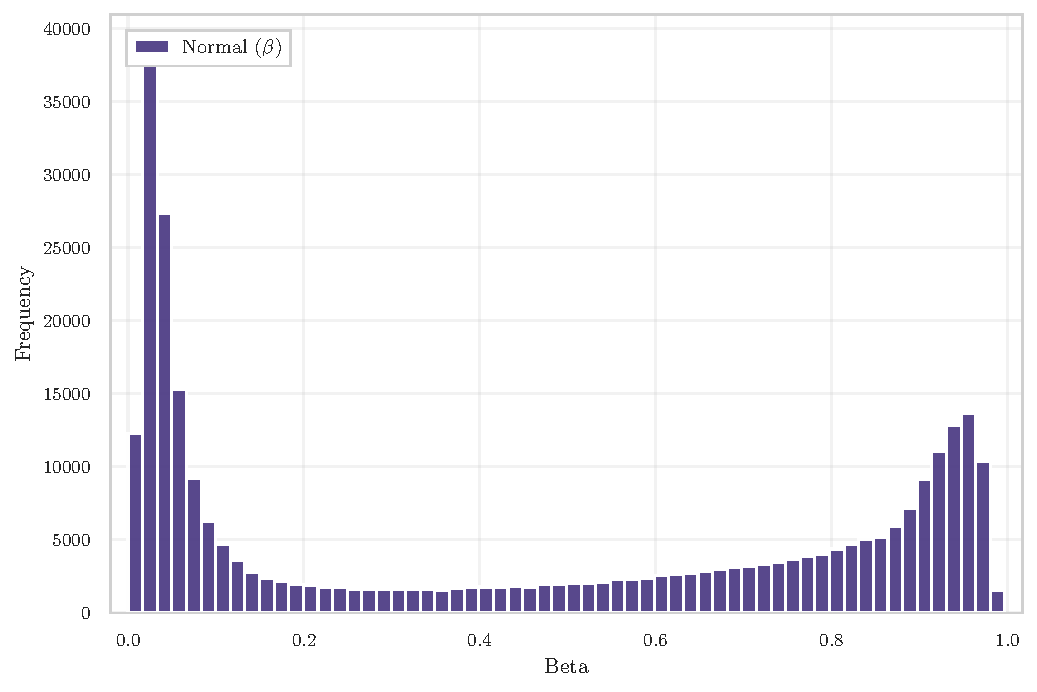
\includegraphics[width=\textwidth]{images/cap4/GSE69914_hist_normal_beta.pdf}
        \caption{Normal ($\beta$)}
    \end{subfigure}
    \begin{subfigure}{0.24\textwidth}
        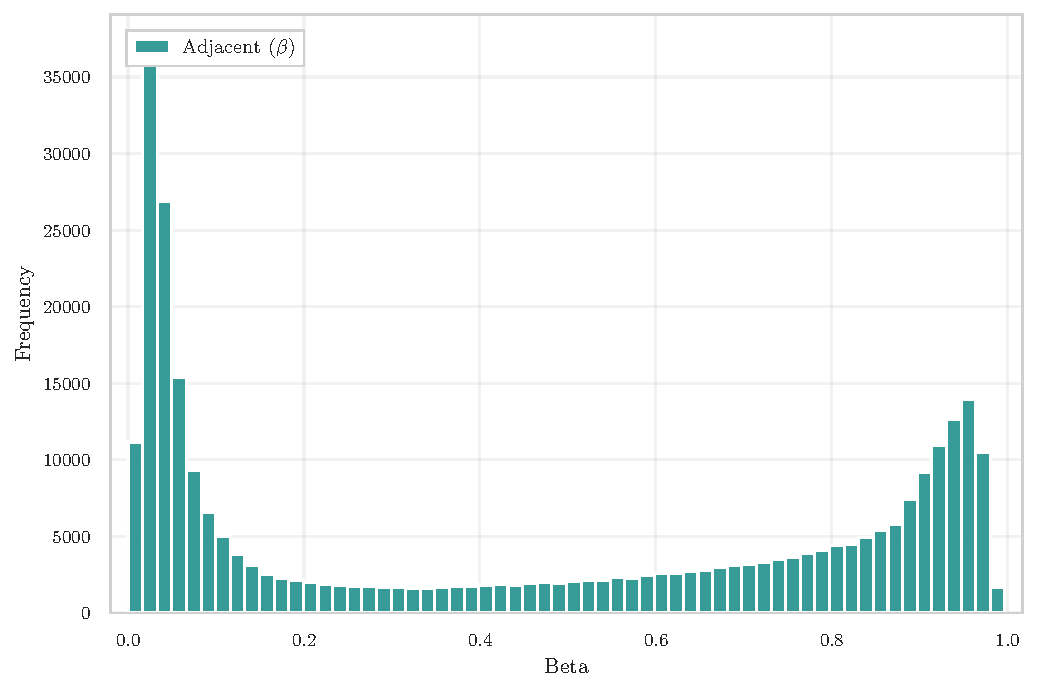
\includegraphics[width=\textwidth]{images/cap4/GSE69914_hist_adjacent_beta.pdf}
        \caption{Adjacent ($\beta$)}
    \end{subfigure}
    \begin{subfigure}{0.24\textwidth}
        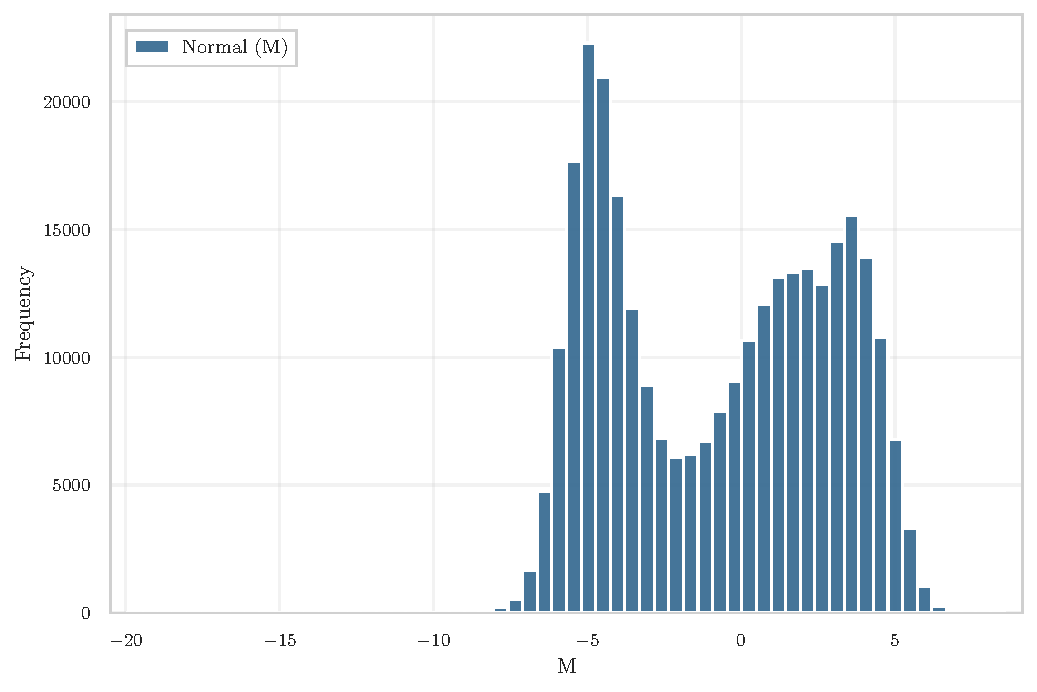
\includegraphics[width=\textwidth]{images/cap4/GSE69914_hist_normal_m.pdf}
        \caption{Normal ($M$)}
    \end{subfigure}
    \begin{subfigure}{0.24\textwidth}
        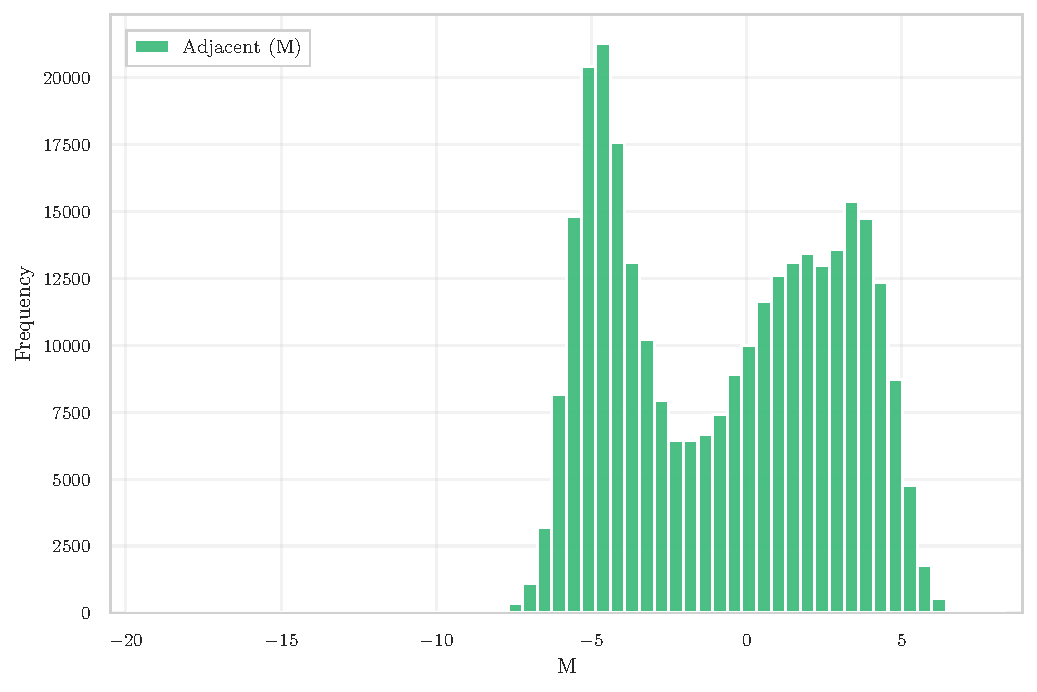
\includegraphics[width=\textwidth]{images/cap4/GSE69914_hist_adjacent_m.pdf}
        \caption{Adjacent ($M$)}
    \end{subfigure}

    \vspace{0.8em}

    % ---------------- ROW 2: MEAN–SD RELATIONS ----------------
    \begin{subfigure}{0.24\textwidth}
        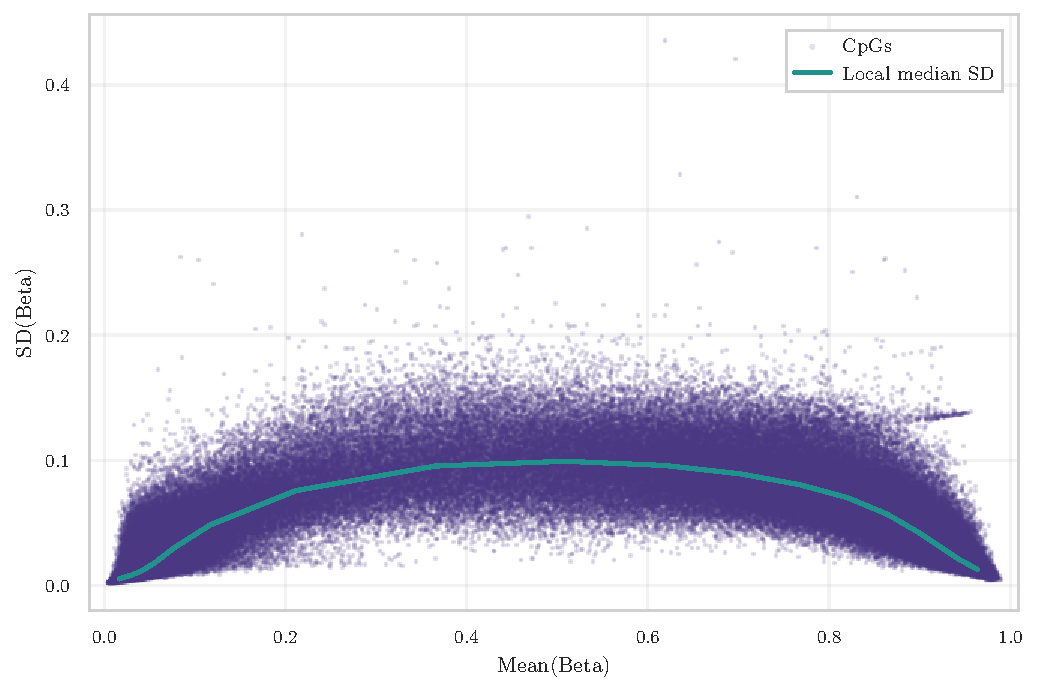
\includegraphics[width=\textwidth]{images/cap4/GSE69914_msd_normal_beta.pdf}
        \caption{Mean–SD Normal ($\beta$)}
    \end{subfigure}
    \begin{subfigure}{0.24\textwidth}
        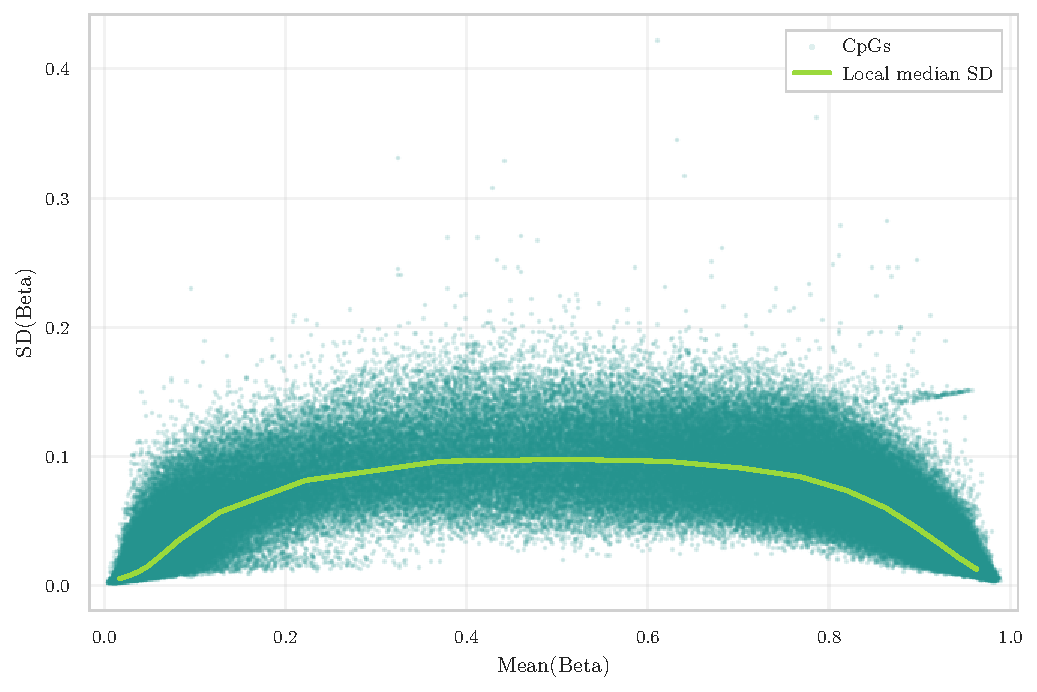
\includegraphics[width=\textwidth]{images/cap4/GSE69914_msd_adjacent_beta.pdf}
        \caption{Mean–SD Adjacent ($\beta$)}
    \end{subfigure}
    \begin{subfigure}{0.24\textwidth}
        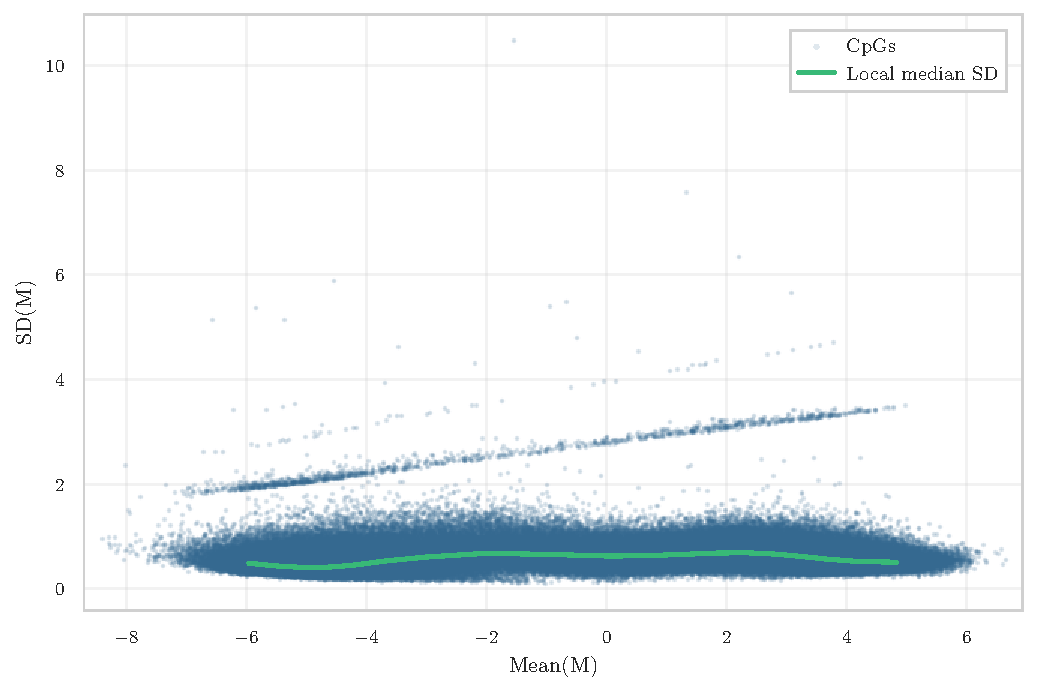
\includegraphics[width=\textwidth]{images/cap4/GSE69914_msd_normal_m.pdf}
        \caption{Mean–SD Normal ($M$)}
    \end{subfigure}
    \begin{subfigure}{0.24\textwidth}
        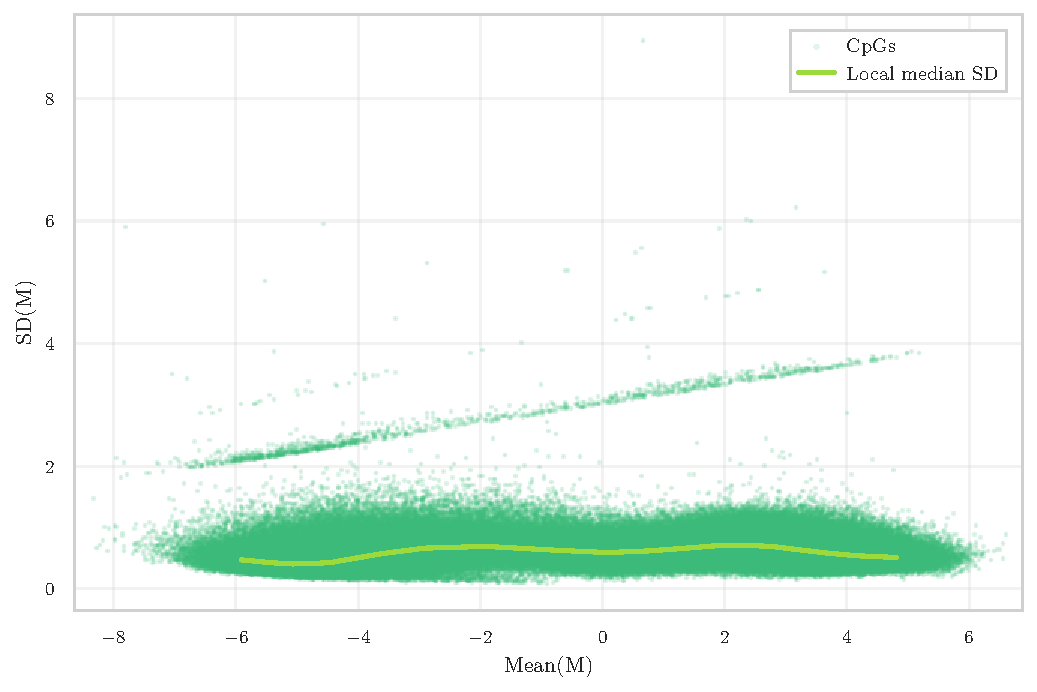
\includegraphics[width=\textwidth]{images/cap4/GSE69914_msd_adjacent_m.pdf}
        \caption{Mean–SD Adjacent ($M$)}
    \end{subfigure}

    \caption{Distributional comparison of $\beta$ and $M$ in Normal and Adjacent tissues in GSE69914.}
    \label{fig:hist_msd_beta_m}
\end{figure}

Following transformation, the empirical distributions confirm the expected variance-stabilising behaviour of $M$-values (Figure~\ref{fig:hist_msd_beta_m}). In $\beta$-space, both Normal and Adjacent tissues exhibit the characteristic bounded, U-shaped distribution with accumulation near 0 and 1. After logit transformation, the corresponding $M$-value distributions become substantially more symmetric and centered, while preserving the relative structure between tissue groups.
The mean–SD relationships further illustrate the scale effect. In $\beta$-space, variance is strongly mean-dependent and inflates near intermediate methylation levels, producing a pronounced curvature in the mean–SD plots. In contrast, $M$-values display markedly flatter dispersion profiles across the full range, indicating substantial reduction of heteroscedasticity. 
This behaviour is fully consistent with the theoretical and empirical findings of Du et al.~\cite{Du2010}, which motivate the use of $M$-values for inferential modelling.


% ============================================================

\subsection{Dataset GSE225845}
\label{subsec:gse225845_preproc}
% ============================================================

\paragraph{Structural Integrity and Cohort Harmonization}
\label{par:gse225845_step0}

The dataset comprised 477 samples and 750{,}426 CpGs at load time, consistent with the dimensionality of the Illumina EPIC platform.  
The phenotype table contained 477 entries, and alignment between phenotype annotation and the $\beta$-value matrix was exact. No duplicated entries were detected, and all required metadata fields were present.
Probe-level and sample-level missingness assessment confirmed that the methylation matrix was fully observed.  
No missing CpG values and no incomplete samples were detected. Consequently, no imputation or early NaN filtering was required prior to probe-type bias diagnostics and technical filtering.


\paragraph{Probe-Type Bias Diagnostics and Correction}
\label{par:gse225845_step1}
\begin{figure}[t]
    \centering
    \begin{subfigure}[t]{0.48\linewidth}
        \centering
        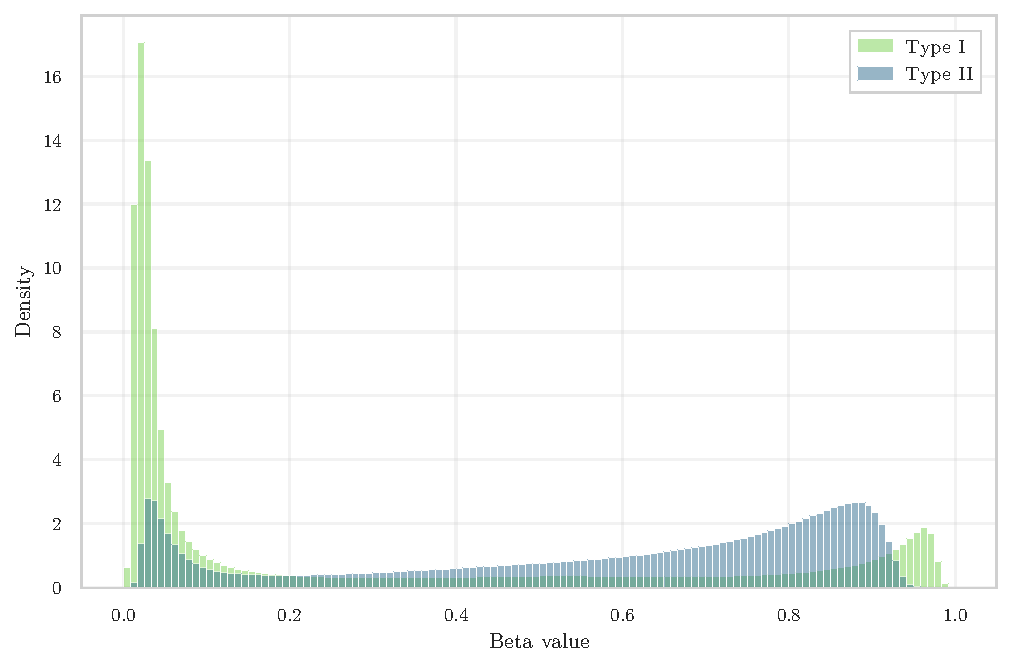
\includegraphics[height=4.5cm,keepaspectratio]{images/cap4/GSE225845_type_bias_density.pdf}
        \caption{$\beta$-value density by probe type.}
        \label{fig:GSE225845_type_bias_density}
    \end{subfigure}
    \hfill
    \begin{subfigure}[t]{0.48\linewidth}
        \centering
        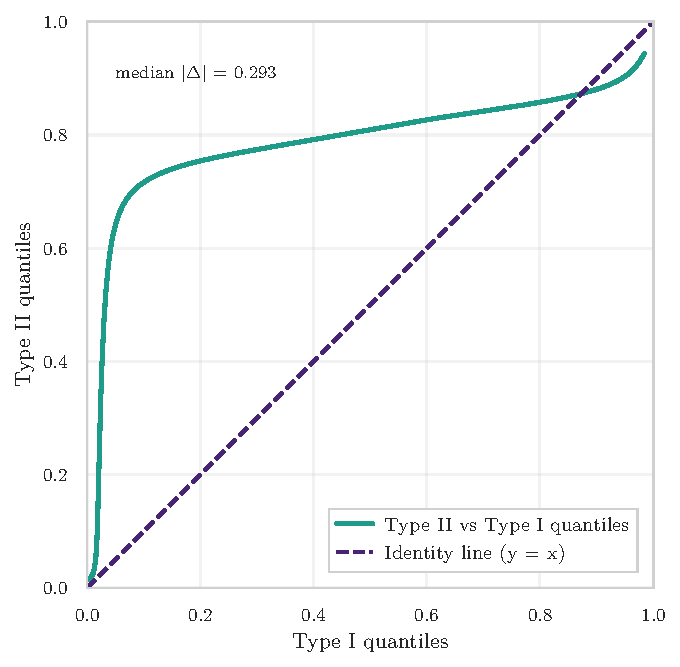
\includegraphics[height=4.5cm,keepaspectratio]{images/cap4/GSE225845_type_bias_qqplot.pdf}
        \caption{Q--Q plot (Type~II vs.~Type~I).}
        \label{fig:GSE225845_type_bias_qq}
    \end{subfigure}
    \caption{Infinium Type~I/II bias diagnostics in GSE225845.}
    \label{fig:type_bias_combined}
\end{figure}

Stratification by probe design yielded 119{,}760 Type~I and 627{,}842 Type~II probes.  
Raw intensity data were reported by the original authors to have been processed using the \texttt{minfi} pipeline with BMIQ normalization (v1.4)~\cite{GSE225845}.
The $\beta$-value density distributions (Figure~\ref{fig:GSE225845_type_bias_density}) show substantial overlap between probe families. Type~I probes retain the characteristic concentration near the unmethylated and fully methylated boundaries, while Type~II probes display a broader distribution; however, no pronounced multimodal distortion or systematic separation is observed.
Quantile--quantile analysis (Figure~\ref{fig:GSE225845_type_bias_qq}) further supports this interpretation. Although minor deviations from the identity line ($y = x$) are visible, the overall alignment indicates largely balanced probe-type scaling. The median absolute deviation $\mathrm{median}|\Delta| = 0.293$ suggests that probe-type differences are attenuated but not entirely eliminated, consistent with residual variation commonly observed after BMIQ normalization~\cite{Teschendorff2013BMIQ, maksimovic2012, Wang2015Normalization450K}.
Overall, the diagnostic patterns are compatible with prior application of probe-type bias correction.

\paragraph{Technical Probe Filtering}
\label{par:gse225845_step2}

\begin{figure}[t]
    \centering

    % Panel (a)
    \begin{subfigure}[t]{0.48\linewidth}
        \centering
        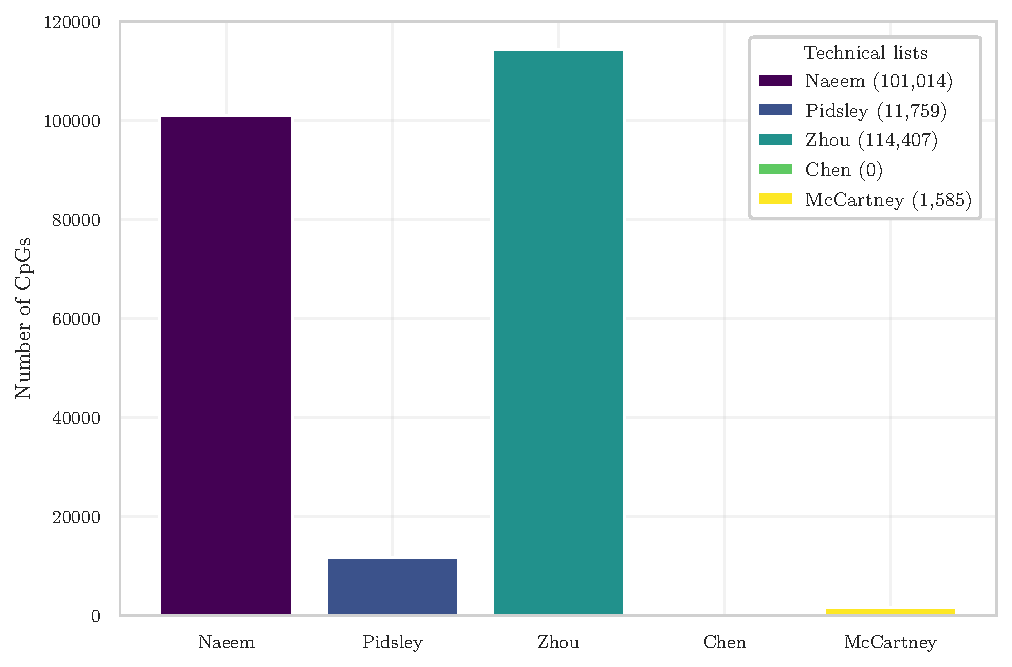
\includegraphics[width=\linewidth]{images/cap4/GSE225845_technical_lists_histogram.pdf}
        \caption{
            CpGs flagged by each technical list. 
        }
        \label{fig:gse225845_tech_barplot}
    \end{subfigure}
    \hfill
    % Panel (b)
    \begin{subfigure}[t]{0.48\linewidth}
        \centering
        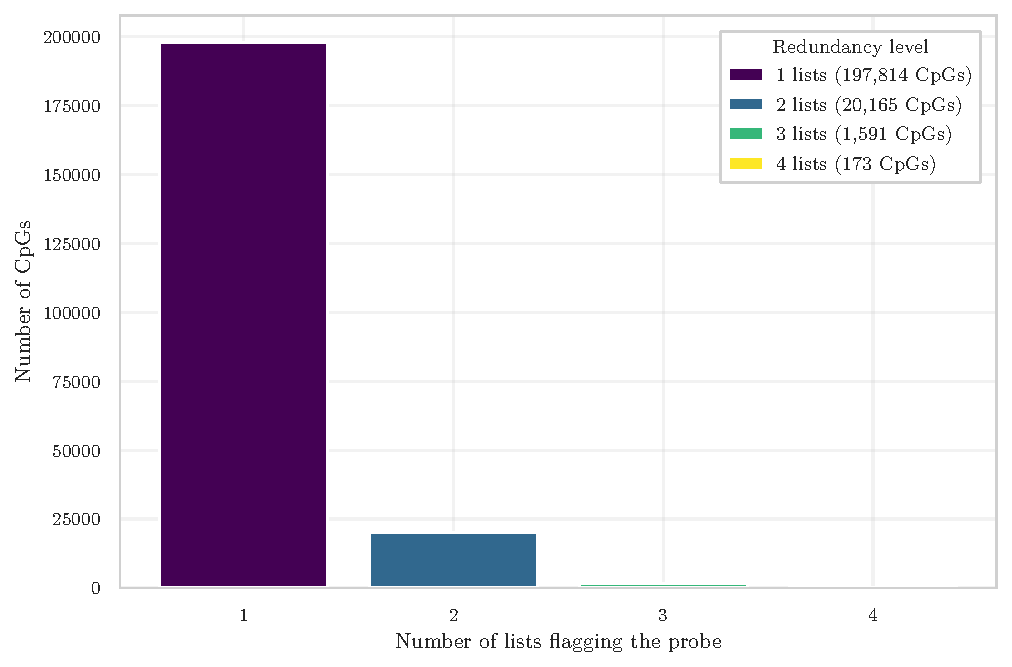
\includegraphics[width=\linewidth]{images/cap4/GSE225845_technical_lists_redundancy_histogram.pdf}
        \caption{Redundancy across filtering lists.}
        \label{fig:gse225845_tech_redundancy}
    \end{subfigure}

    \caption{Technical filtering summary in GSE225845.}
    \label{fig:gse225845_technical_filtering}
\end{figure}

Intersection with external technical filtering resources resulted in substantial probe removal, as summarised in Table~\ref{tab:gse225845_cpg_filtering}. The largest individual contributions derive from the Zhou and Naeem annotations, while the remaining resources flag smaller subsets. The redundancy structure across lists is shown in Figure~\ref{fig:gse225845_tech_redundancy}.
A detailed per-probe exclusion summary is available in the project repository at  
\href{https://github.com/elisabettaroviera/THESIS/blob/main/05%20-%20CpG%20list/Removed%20CpGs%20per%20Dataset/removed_cpgs_all_filters_summary_gse225845.csv}
{\texttt{removed\_cpgs\_all\_filters\_summary\_gse225845.csv}}.
\begin{table}[t]
\centering
\caption{CpG filtering summary for the GSE225845 dataset.}
\label{tab:gse225845_cpg_filtering}
\scriptsize
\begin{tabular}{c c c c c c c c c}
\toprule
Initial CpGs &
Naeem &
Pidsley &
Zhou &
Chen &
McCartney &
Non-CpG &
X/Y &
Final CpGs \\
\midrule
750{,}426 &
101{,}014 &
11{,}759 &
114{,}407 &
0 &
1{,}585 &
773 &
14{,}071 &
530{,}683 \\
\bottomrule
\end{tabular}
\end{table}

\paragraph{Statistical Transformation: $\beta$-to-$M$ Values}
\label{par:gse225845_step3}

\begin{figure}[t]
    \centering

    % ---------------- ROW 1: HISTOGRAMS ----------------
    \begin{subfigure}{0.24\textwidth}
        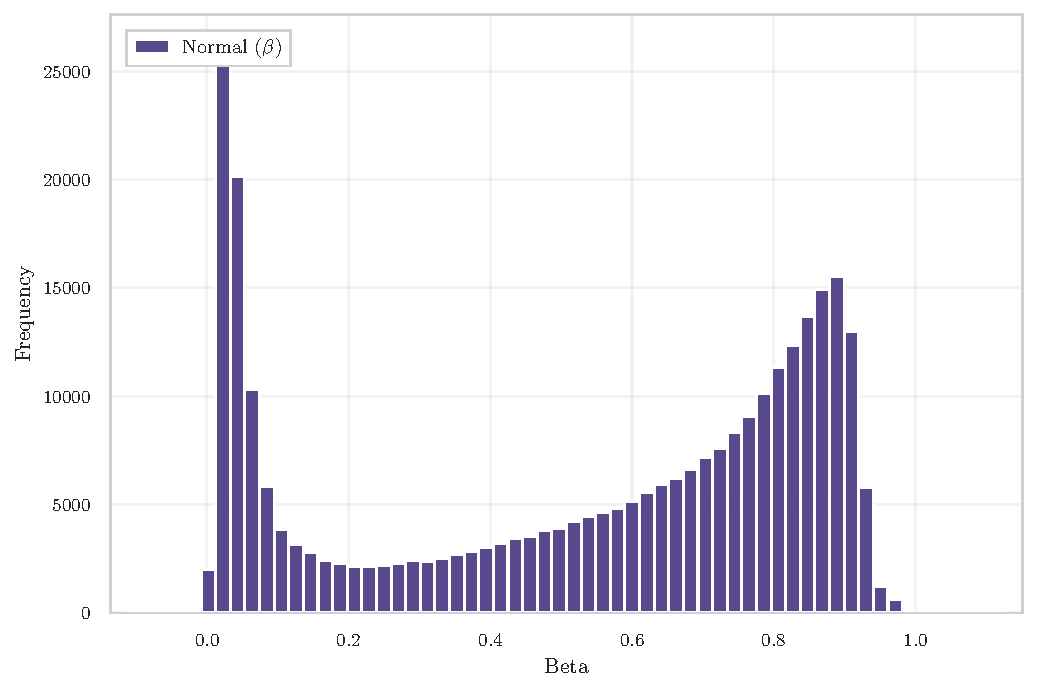
\includegraphics[width=\textwidth]{images/cap4/GSE225845_hist_normal_beta.pdf}
        \caption{Normal ($\beta$)}
    \end{subfigure}
    \begin{subfigure}{0.24\textwidth}
        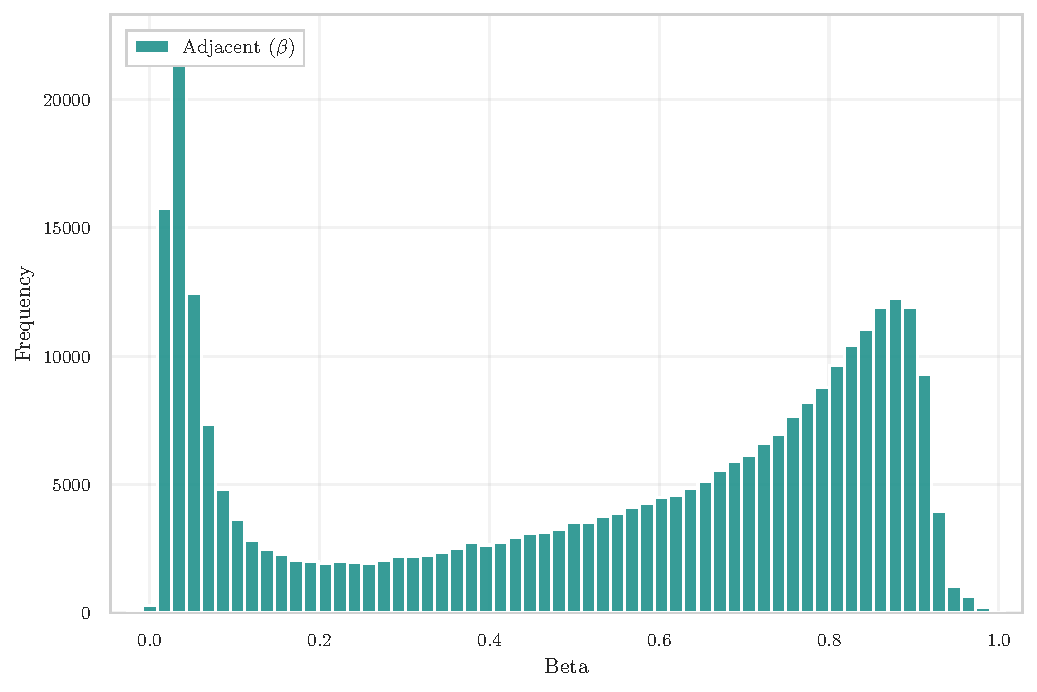
\includegraphics[width=\textwidth]{images/cap4/GSE225845_hist_adjacent_beta.pdf}
        \caption{Adjacent ($\beta$)}
    \end{subfigure}
    \begin{subfigure}{0.24\textwidth}
        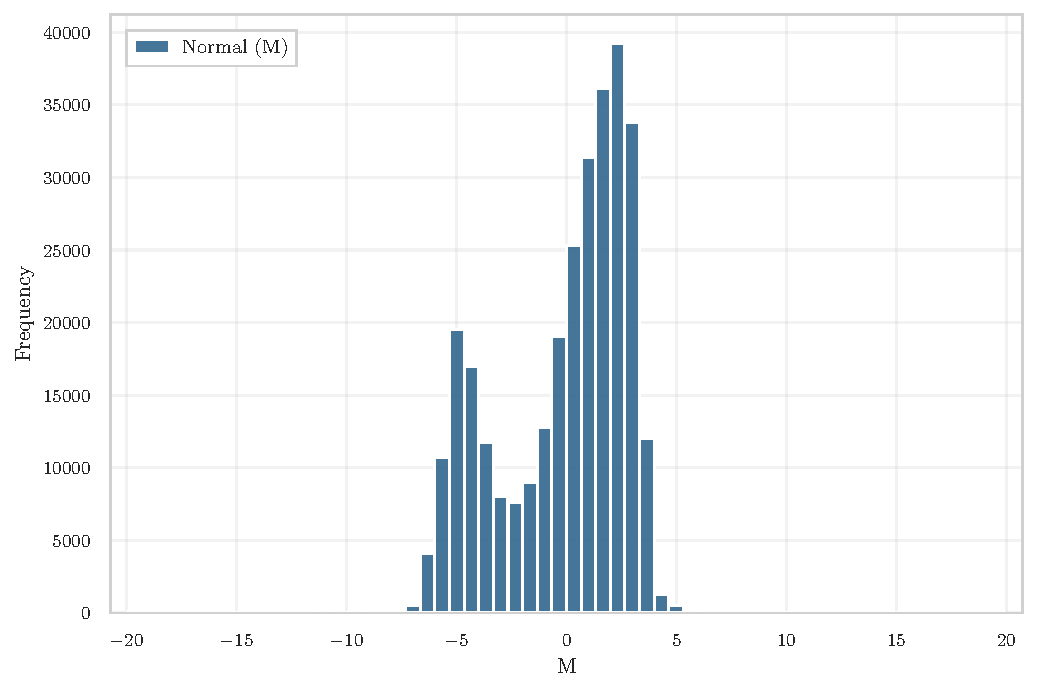
\includegraphics[width=\textwidth]{images/cap4/GSE225845_hist_normal_m.pdf}
        \caption{Normal ($M$)}
    \end{subfigure}
    \begin{subfigure}{0.24\textwidth}
        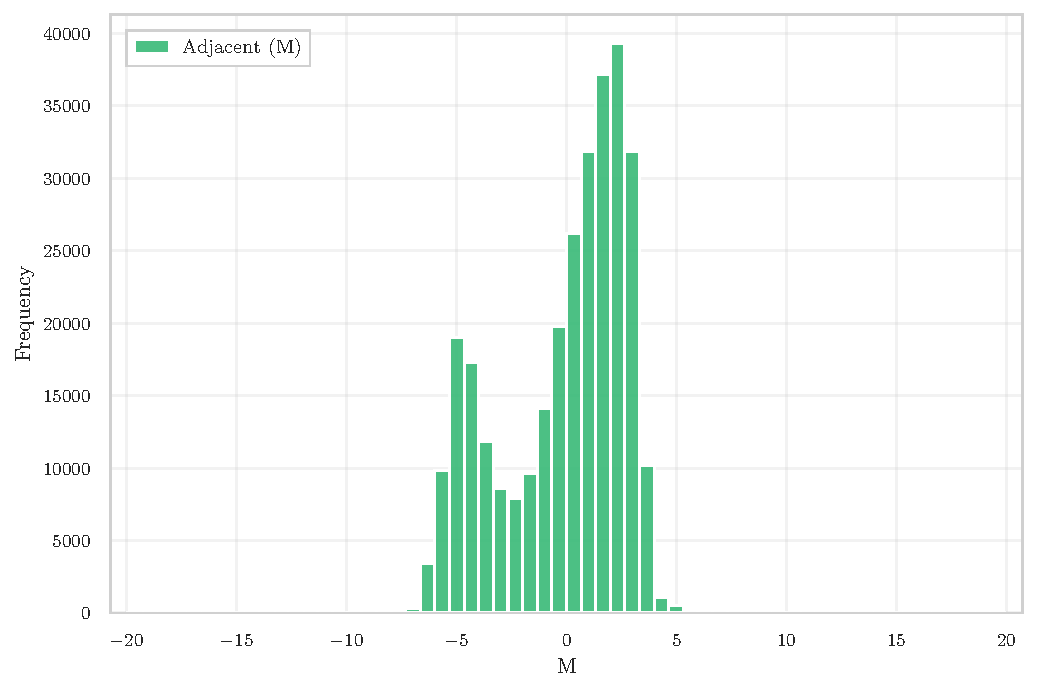
\includegraphics[width=\textwidth]{images/cap4/GSE225845_hist_adjacent_m.pdf}
        \caption{Adjacent ($M$)}
    \end{subfigure}

    \vspace{0.3cm}

    % ---------------- ROW 2: MEAN–SD RELATIONS ----------------
    \begin{subfigure}{0.24\textwidth}
        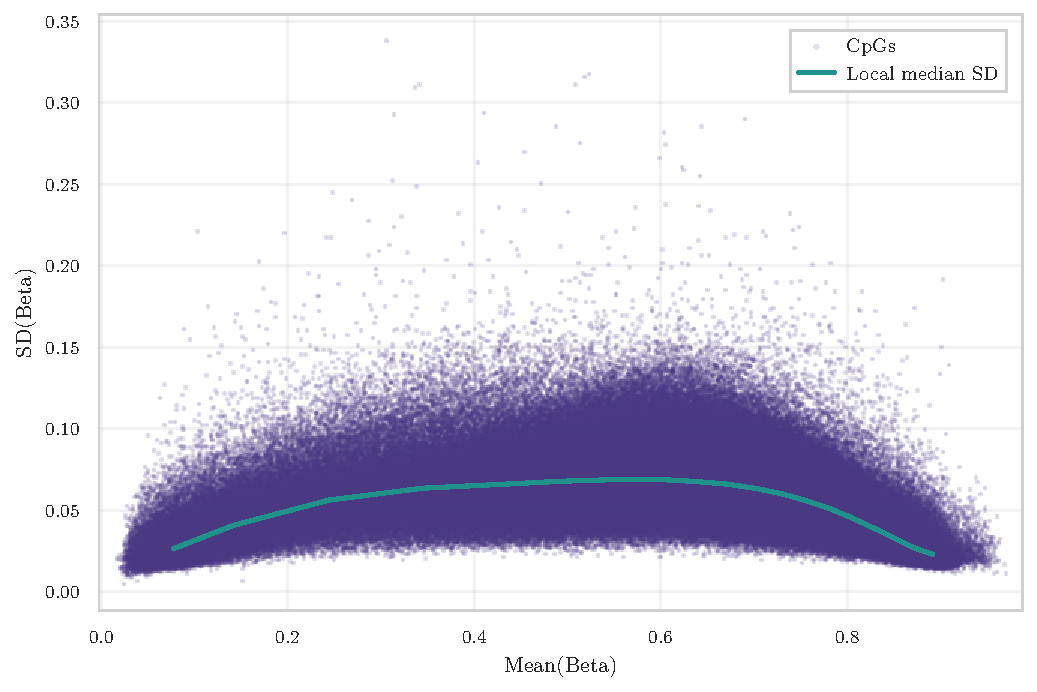
\includegraphics[width=\textwidth]{images/cap4/GSE225845_msd_normal_beta.pdf}
        \caption{Mean–SD Normal ($\beta$)}
    \end{subfigure}
    \begin{subfigure}{0.24\textwidth}
        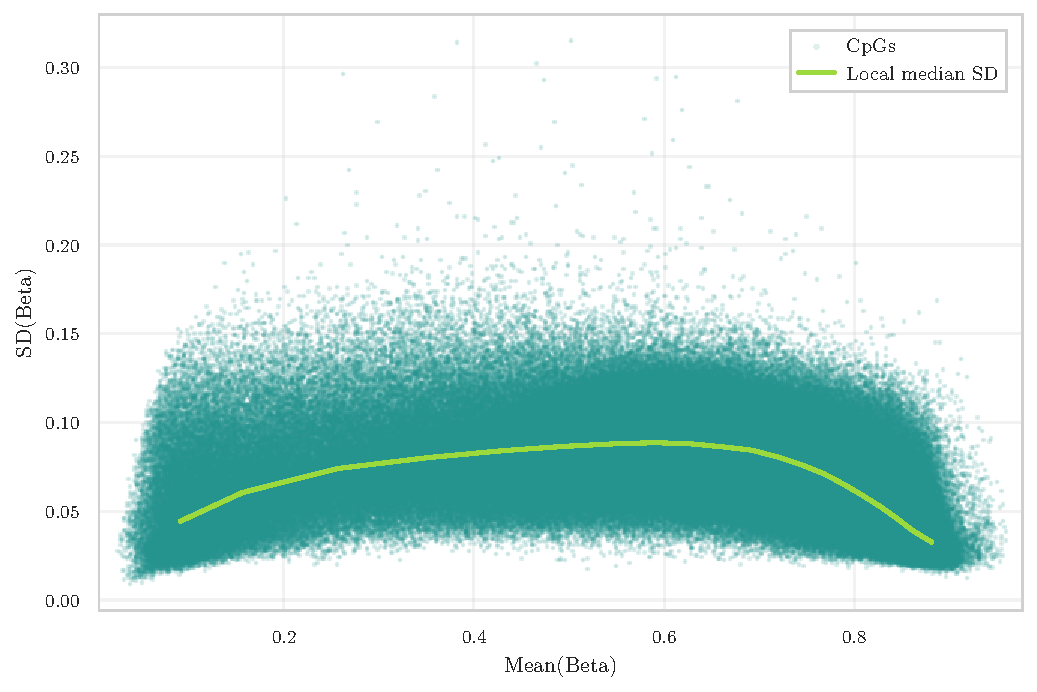
\includegraphics[width=\textwidth]{images/cap4/GSE225845_msd_adjacent_beta.pdf}
        \caption{Mean–SD Adjacent ($\beta$)}
    \end{subfigure}
    \begin{subfigure}{0.24\textwidth}
        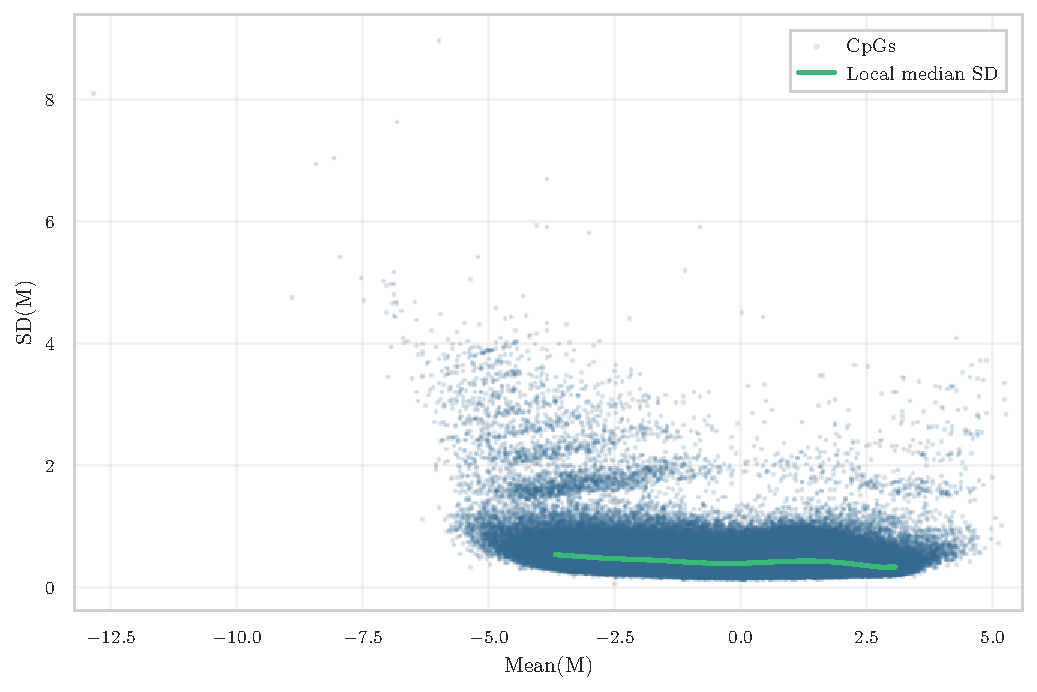
\includegraphics[width=\textwidth]{images/cap4/GSE225845_msd_normal_m.pdf}
        \caption{Mean–SD Normal ($M$)}
    \end{subfigure}
    \begin{subfigure}{0.24\textwidth}
        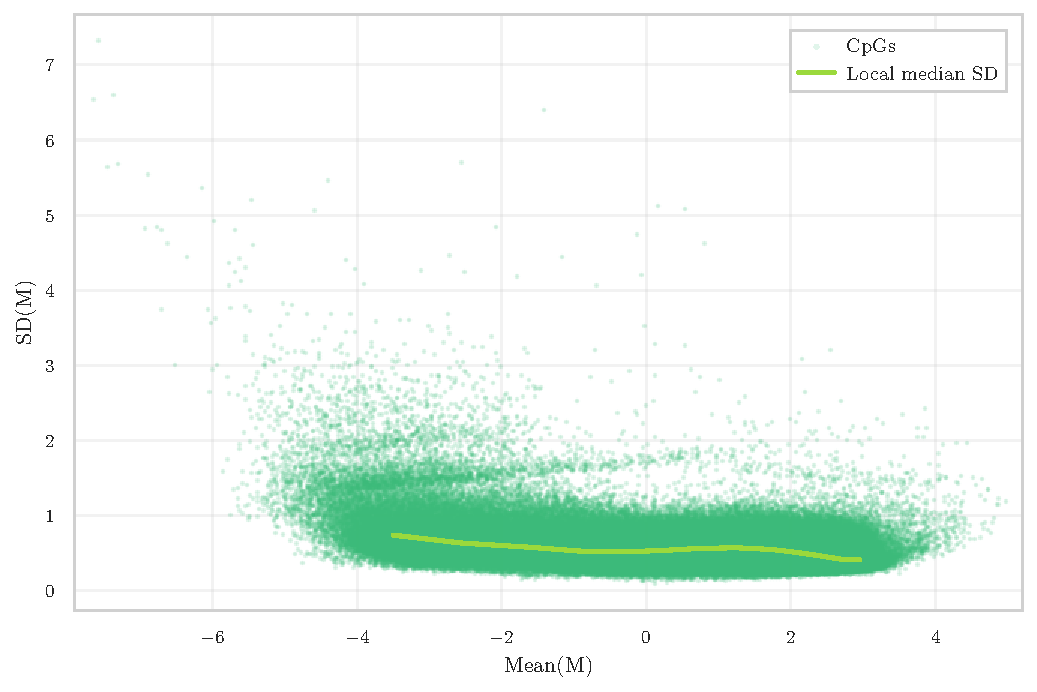
\includegraphics[width=\textwidth]{images/cap4/GSE225845_msd_adjacent_m.pdf}
        \caption{Mean–SD Adjacent ($M$)}
    \end{subfigure}

    \caption{Distributional comparison of $\beta$ and $M$ in Normal and Adjacent
tissues in GSE225845.}
    \label{fig:gse225845_beta_m_combined}
\end{figure}

All filtered $\beta$-values were transformed to $M$-values using the logit relation defined in Equation~\eqref{eq:mvalue}. 
The empirical distributions (Figure~\ref{fig:gse225845_beta_m_combined}) show the characteristic bounded, U-shaped profile in $\beta$-space for both Normal and Adjacent tissues. After transformation, the corresponding $M$-value distributions become substantially more symmetric and centered, while maintaining the relative structure between tissue classes.
The mean--SD relationships further illustrate the scale effect. In $\beta$-space, variance exhibits pronounced mean dependence, with inflation at intermediate methylation levels and compression near the boundaries. In contrast, $M$-values display markedly flatter dispersion profiles across the full range, indicating substantial reduction of heteroscedasticity. 


% ============================================================

\subsection{Dataset GSE287331}
\label{subsec:gse287331_data_prep}
% ============================================================



\paragraph{Structural Integrity and Cohort Harmonization}
\label{par:gse287331_missingness}

The dataset was imported from its Parquet representation, yielding an initial
$\beta$-value matrix of 446 samples and 866{,}552 CpGs. The phenotype table
contained the same number of entries, with all required metadata fields present
and alignment between phenotype annotation and the $\beta$-value matrix exact.
Unlike GSE69914 and GSE225845, the methylation matrix was not fully observed.
Probe-wise missingness is a well-known source of unreliability in Illumina
methylation arrays: Islam \textit{et al.}~\cite{islam2019_pediatric_dnamm}
excluded probes with missing $\beta$-values in more than $2\%$ of samples,
while Mansell \textit{et al.}~\cite{mansell2019guidance} applied a stricter
$1\%$ threshold for detection failure in their EPIC-array quality control
pipeline. Consistent with these recommendations, all CpG sites missing in more
than $1\%$ of samples were removed, prioritising high-confidence measurements
while minimising reliance on imputed values and leveraging the large
dimensionality of the EPIC platform. After applying this criterion, the
remaining sparsity was negligible: 58{,}561 NaN values, corresponding to
$0.0187\%$ of all entries. Given this extremely low level of sparsity,
median-based imputation is both statistically robust and
distribution-preserving; residual missing values were therefore imputed using
the probe-wise median $\beta$-value across samples, a strategy that avoids
introducing group-specific bias and is consistent with recent harmonisation
workflows such as mLiftOver, where missing values are explicitly replaced by
probe-wise median substitution to preserve biologically plausible
levels~\cite{chen2024_mliftover}.

After harmonising phenotype labels and applying dataset-specific selection
rules, only samples belonging to the three core tissue states of
interest---Normal, Adjacent, and Tumour---were retained. The final working
matrix consisted of 311 samples and 702{,}916 CpGs, with no residual missing
values.



\begin{figure}[t]
    \centering
    \begin{subfigure}[t]{0.48\linewidth}
        \centering
        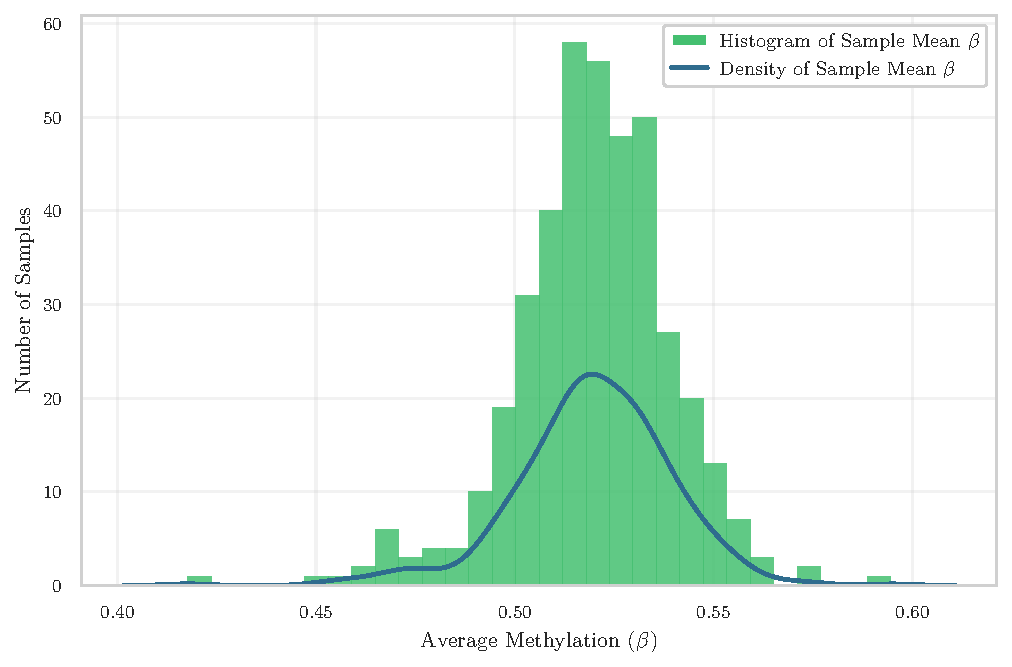
\includegraphics[width=\textwidth,keepaspectratio]{images/cap3/GSE69914_08_mean_beta_per_sample.pdf}
        \caption{GSE69914}
    \end{subfigure}
    \hfill
    \begin{subfigure}[t]{0.48\linewidth}
        \centering
        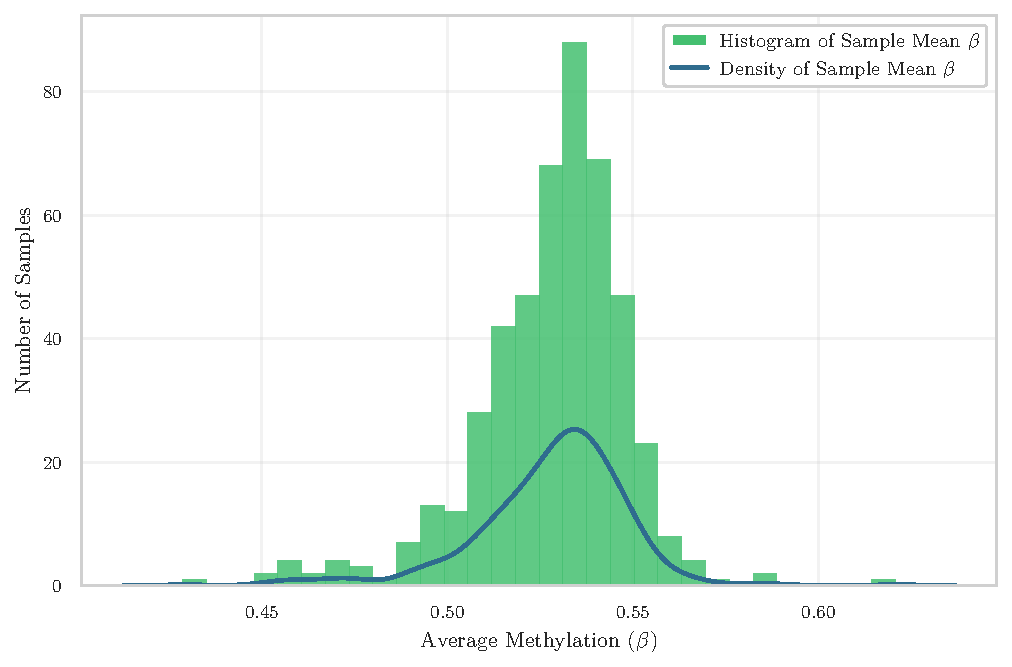
\includegraphics[width=\textwidth,keepaspectratio]{images/cap3/GSE225845_08_mean_beta_per_sample.pdf}
        \caption{GSE225845}
    \end{subfigure}

    \medskip

    \begin{subfigure}[t]{0.48\linewidth}
        \centering
        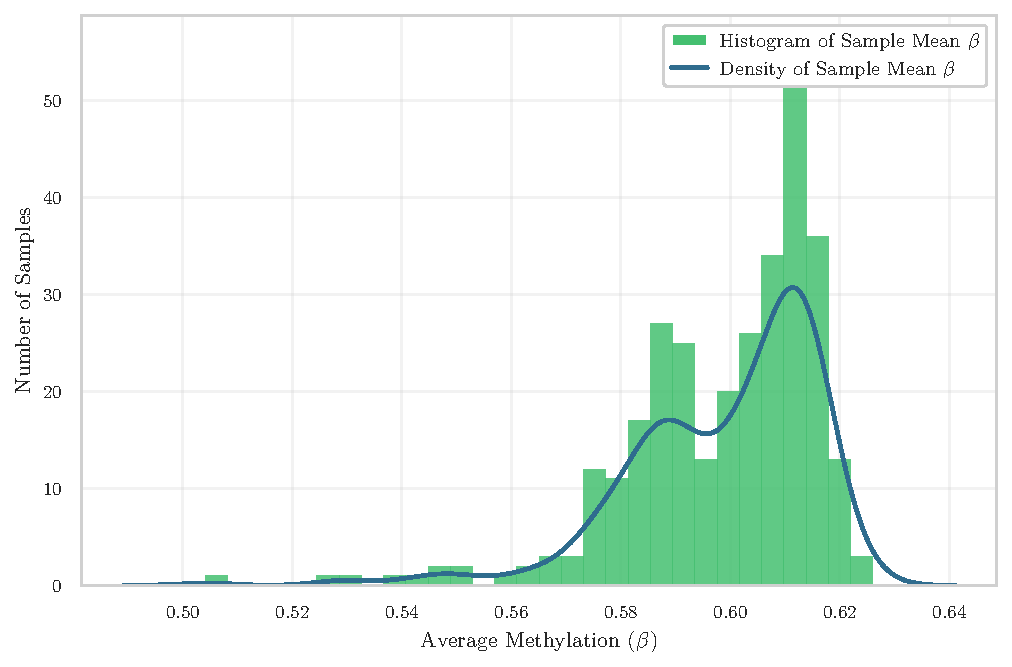
\includegraphics[width=\textwidth,keepaspectratio]{images/cap3/GSE287331_08_mean_beta_per_sample.pdf}
        \caption{GSE287331 pre BMIQ}
    \end{subfigure}
    \hfill
    \begin{subfigure}[t]{0.48\linewidth}
        \centering
        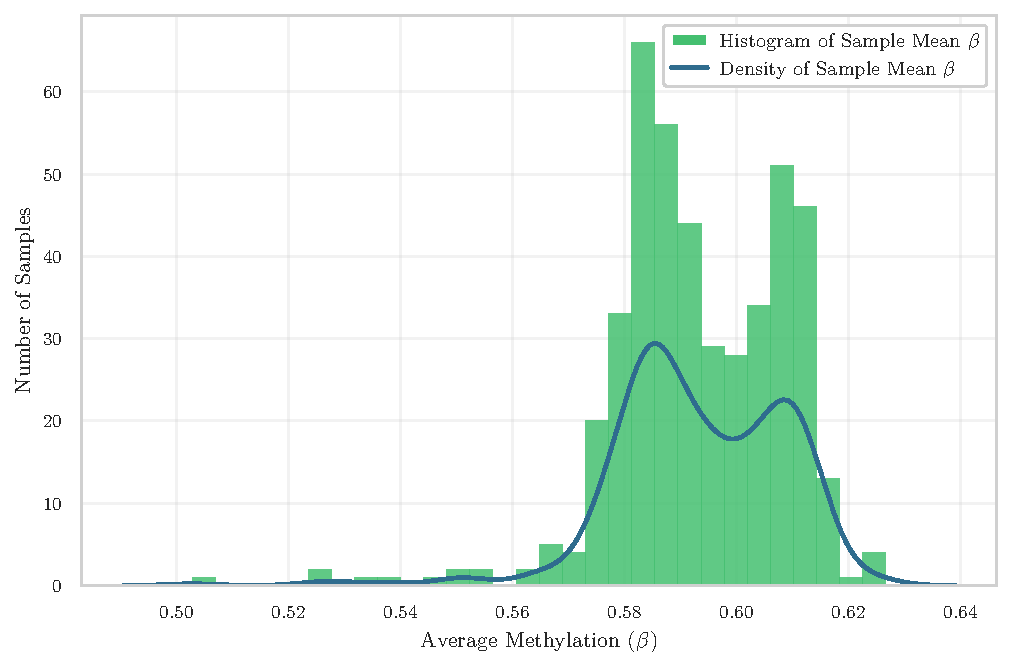
\includegraphics[width=\textwidth,keepaspectratio]{images/cap3/GSE287331_03_mean_beta_per_sample.pdf}
        \caption{GSE287331 post BMIQ}
    \end{subfigure}
    \caption{Per-sample mean $\beta$ distributions for the three datasets.}
\end{figure}

\begin{figure}[t]
    \centering

    % -------- Row 1: first two subfigures side by side --------
    \begin{subfigure}[t]{0.48\linewidth}
        \centering
        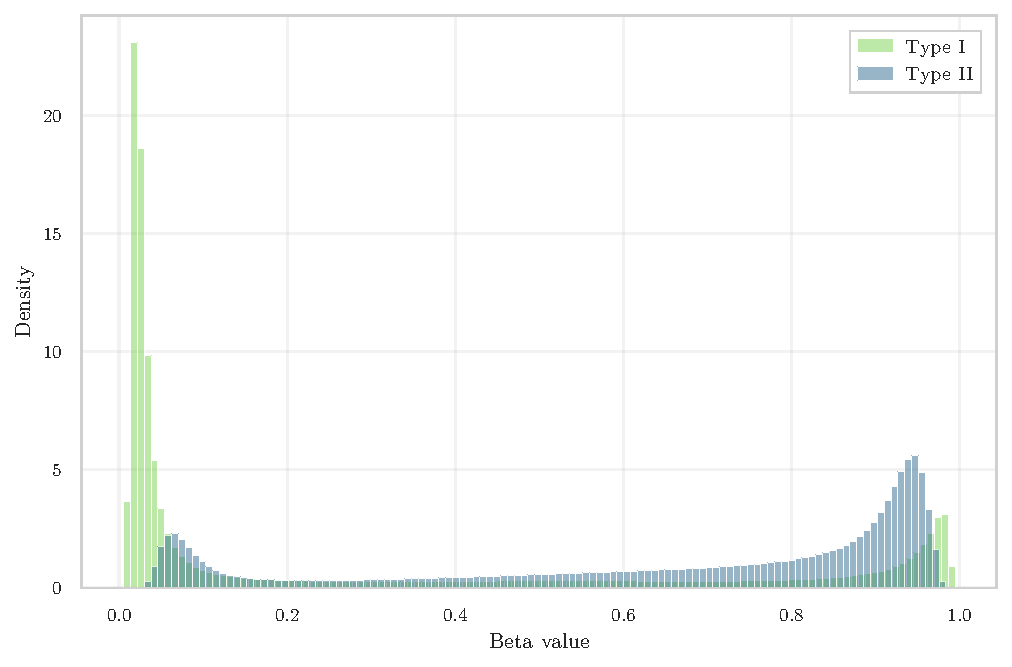
\includegraphics[height=4.5cm,keepaspectratio]{images/cap3/GSE287331_23_type_bias_density_pre.pdf}
        \caption{GSE287331 pre BMIQ}
        \label{fig:gse287331_typeI_II_pre}
    \end{subfigure}
    \hfill
    \begin{subfigure}[t]{0.48\linewidth}
        \centering
        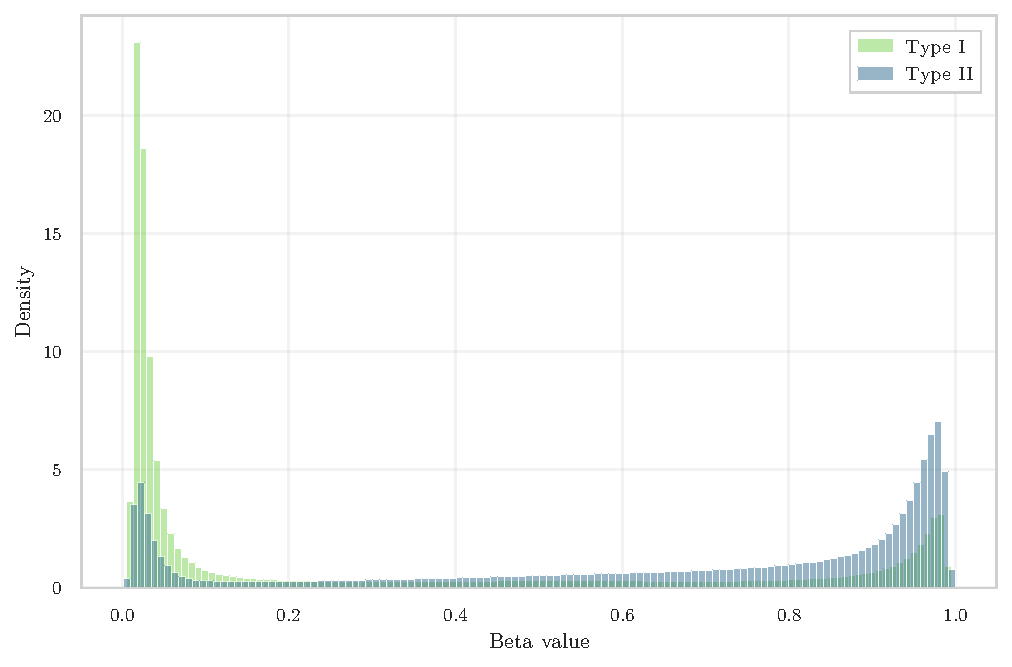
\includegraphics[height=4.5cm,keepaspectratio]{images/cap3/GSE287331_23_type_bias_density_post.pdf}
        \caption{GSE287331 post BMIQ}
        \label{fig:gse287331_typeI_II_post}
    \end{subfigure}

    \medskip

    % -------- Row 2: third subfigure centred --------
    \begin{subfigure}[t]{0.48\linewidth}
        \centering
        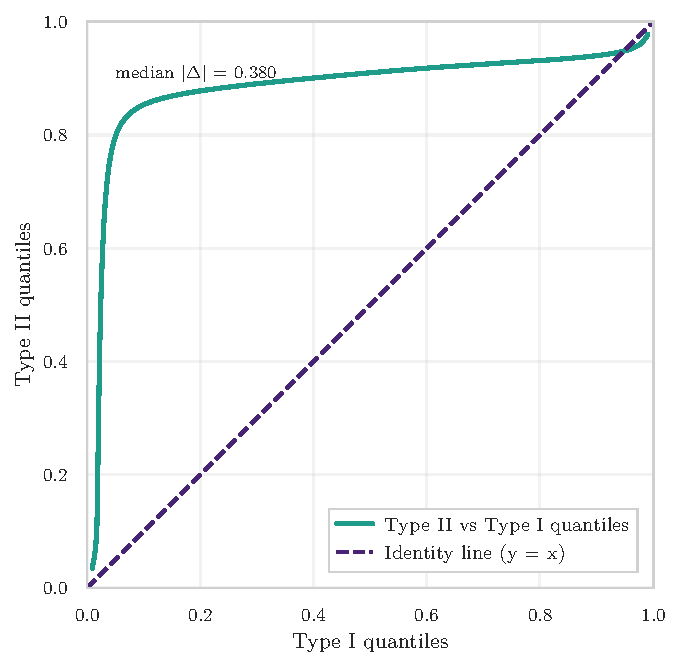
\includegraphics[height=4.5cm,keepaspectratio]{images/cap4/GSE287331_type_bias_qqplot.pdf}
        \caption{Q--Q comparison of Type~II vs.\ Type~I probes (pre BMIQ).}
        \label{fig:gse287331_type_bias_qq}
    \end{subfigure}

    \caption{Infinium Type~I/II bias diagnostics in GSE287331. Pre-BMIQ
      densities and Q--Q analysis indicate marked probe-type imbalance;
      post-BMIQ densities show partial alignment.}
    \label{fig:mean_beta_comparison_three}
\end{figure}

\paragraph{Probe-Type Bias Diagnostics and Correction}
\label{subpar:gse287331_typebias}



Using the official EPIC v1.0 manifest, 115{,}705 Type~I and 585{,}514 Type~II
probes were identified. Unlike GSE69914 and GSE225845, for which the original
authors reported prior application of BMIQ normalisation, no probe-design bias
correction was documented in the processing pipeline of GSE287331. This absence
was first suggested by the per-sample mean $\beta$-value distributions
(Figure~\ref{fig:mean_beta_comparison_three}): whereas GSE69914 and GSE225845
display a single broad peak, GSE287331 shows a narrower, right-shifted
distribution characterised by two distinct modes in the high-$\beta$ range---a
pattern largely absent in the other cohorts and strongly indicative of uncorrected
Type~I/II probe-design bias.
Stratification of probes by design type confirmed this hypothesis. The
$\beta$-value distributions of the two chemistries showed a marked mismatch
(Figure~\ref{fig:gse287331_typeI_II_pre}), with Type~II probes displaying a
strong right-shifted profile. The quantile--quantile comparison confirmed a
substantial systematic offset, with a median absolute deviation of $0.380$
(Figure~\ref{fig:gse287331_type_bias_qq}), fully incompatible with BMIQ-corrected
data. Inspection of the original publication~\cite{Lord2024GSE287331} further
confirmed the absence of any mention of BMIQ, SWAN, noob, or equivalent
probe-type correction methods.

Given this evidence, the canonical BMIQ algorithm~\cite{Teschendorff2013BMIQ}
was applied using the \texttt{wateRmelon} implementation~\cite{Pidsley2013wateRmelon},
operating strictly on a per-sample basis: Type~I probes define the reference
mixture distribution within each sample, and Type~II probes are rescaled
accordingly, with no cross-sample or cross-group information introduced at any
stage. Samples with insufficient numbers of probes per design type were left
uncorrected to avoid unstable mixture estimation.
Post-correction diagnostics showed only a modest reduction in probe-type mismatch
($|\Delta| : 0.380 \rightarrow 0.370$), with the overall distributional discrepancy
remaining substantial and the bimodality of per-sample mean $\beta$ distributions
persisting (Figure~\ref{fig:mean_beta_comparison_three},
Figure~\ref{fig:gse287331_typeI_II_post}). This limited harmonisation is consistent
with documented caveats of quantile-based normalisation on EPIC arrays, which can
artificially reduce biological variability, remove genuine group-level signal, or
yield distorted distributions when differences are expressed as broad distributional
shifts~\cite{Yousefi2013, Welsh2023EPICnorm, Liu2016Processing}.
The impact on biological structure was assessed quantitatively via silhouette
analysis: the average silhouette coefficient declined from
$\mathrm{sil}_{\text{pre}} = 0.2876 \text{ to } \mathrm{sil}_{\text{post}} = 0.2537$
after correction, indicating that BMIQ reduced the natural clusterability of the
data and collapsed genuine group-level separation---particularly between Normal
and Adjacent samples. For this reason, all downstream analyses are carried out on
the non-BMIQ version of the dataset, which preserves sharper cluster boundaries
and avoids normalisation-induced shrinkage of biological signal.



\paragraph{Technical Probe Filtering}
\label{par:gse287331_step2}



Intersection with external technical filtering resources resulted in substantial probe removal, as summarised in Table~\ref{tab:gse287331_cpg_filtering}. The largest individual contributions derive from the Naeem and Zhou annotations, while the remaining resources flag smaller but non-negligible subsets (Figure~\ref{fig:gse287331_tech_barplot}).  
Importantly, in the unfiltered EPIC matrix the Zhou annotation alone would have excluded 192{,}856 CpGs. This number substantially exceeds the net contribution observed at this stage, indicating that a considerable fraction of Zhou-flagged probes had already been removed during the earlier missingness-cleaning step.
The missingness filter and the Zhou reliability masks therefore exhibit non-trivial overlap. 
This concordance supports the robustness of the preprocessing strategy: probes excluded due to empirical data sparsity largely coincide with loci independently annotated as technically unreliable, suggesting that early NaN-based exclusion was not arbitrary but aligned with established probe-quality criteria.
The redundancy structure across lists (Figure~\ref{fig:gse287331_tech_redundancy}) further indicates that most excluded CpGs are supported by a single resource, with progressively fewer loci flagged by multiple independent annotations.
Annotation-based validation using the MethylationEPIC v1.0 manifest~\cite{IlluminaEPIC} further excluded non-CpG probes and loci lacking reliable genomic annotation. 
Across all filters, the dimensionality reduction is detailed in Table~\ref{tab:gse287331_cpg_filtering}.
A probe-level exclusion summary is available in the project repository at  
\href{https://github.com/elisabettaroviera/THESIS/blob/main/05%20-%20CpG%20list/Removed%20CpGs%20per%20Dataset/removed_cpgs_all_filters_summary_gse287331.csv}
{\texttt{removed\_cpgs\_all\_filters\_summary\_gse287331.csv}}.

\begin{table}[t]
\centering
\caption{CpG filtering summary for the GSE287331 dataset.}
\label{tab:gse287331_cpg_filtering}
\scriptsize
\begin{tabular}{c c c c c c c c c}
\toprule
Initial CpGs &
Naeem &
Pidsley &
Zhou &
Chen &
McCartney &
Non-CpG &
X/Y &
Final CpGs \\
\midrule
866{,}552 &
124{,}511 &
8{,}992 &
102{,}802 &
1{,}730 &
3{,}672 &
500 &
12{,}579 &
486{,}725 \\
\bottomrule
\end{tabular}
\end{table}

\begin{figure}[t]
    \centering
    \begin{subfigure}[t]{0.48\textwidth}
        \centering
        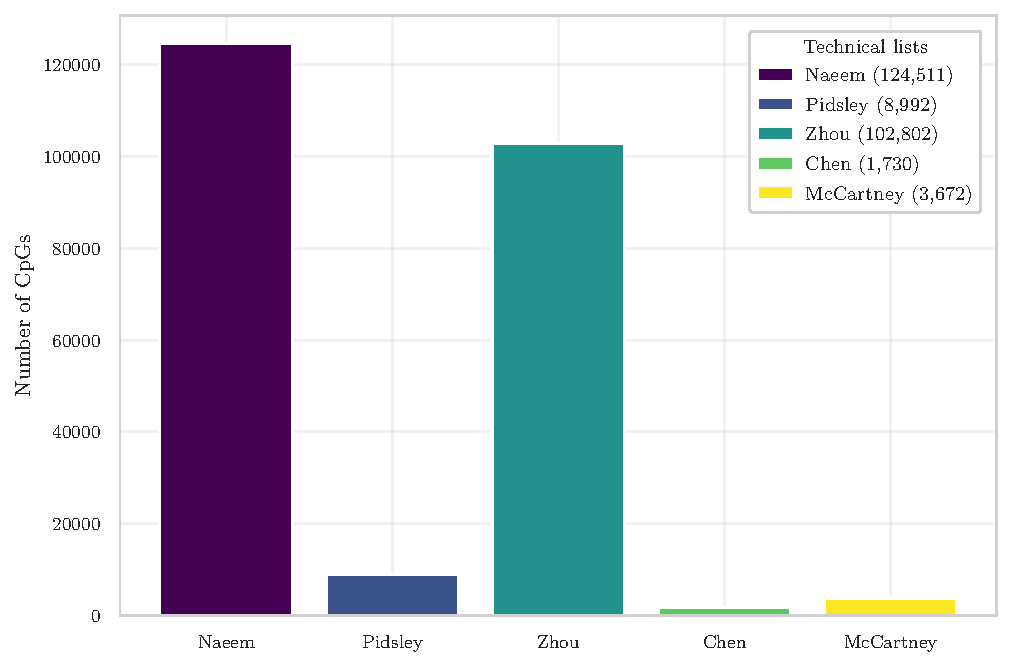
\includegraphics[width=\textwidth]{images/cap4/GSE287331_technical_lists_histogram.pdf}
        \caption{
            CpGs flagged by each technical list.
        }
        \label{fig:gse287331_tech_barplot}
    \end{subfigure}
    \hfill
    \begin{subfigure}[t]{0.48\textwidth}
        \centering
        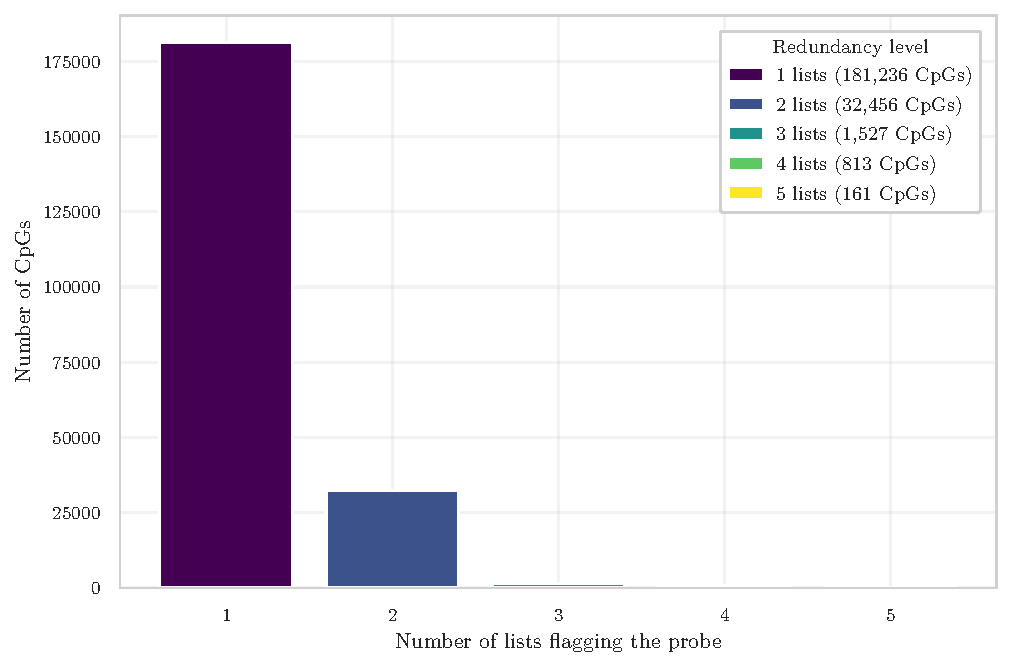
\includegraphics[width=\textwidth]{images/cap4/GSE287331_technical_lists_redundancy_histogram.pdf}
        \caption{
             Redundancy across filtering lists.
        }
        \label{fig:gse287331_tech_redundancy}
    \end{subfigure}
    \caption{Technical filtering summary in GSE287331.}
    \label{fig:gse287331_technical_filtering}
\end{figure}


\paragraph{Statistical Transformation: $\beta$-to-$M$ Values}
\label{par:gse287331_step4}

\begin{figure}[t]
    \centering

    % ---------------- ROW 1: HISTOGRAMS ----------------
    \begin{subfigure}{0.24\textwidth}
        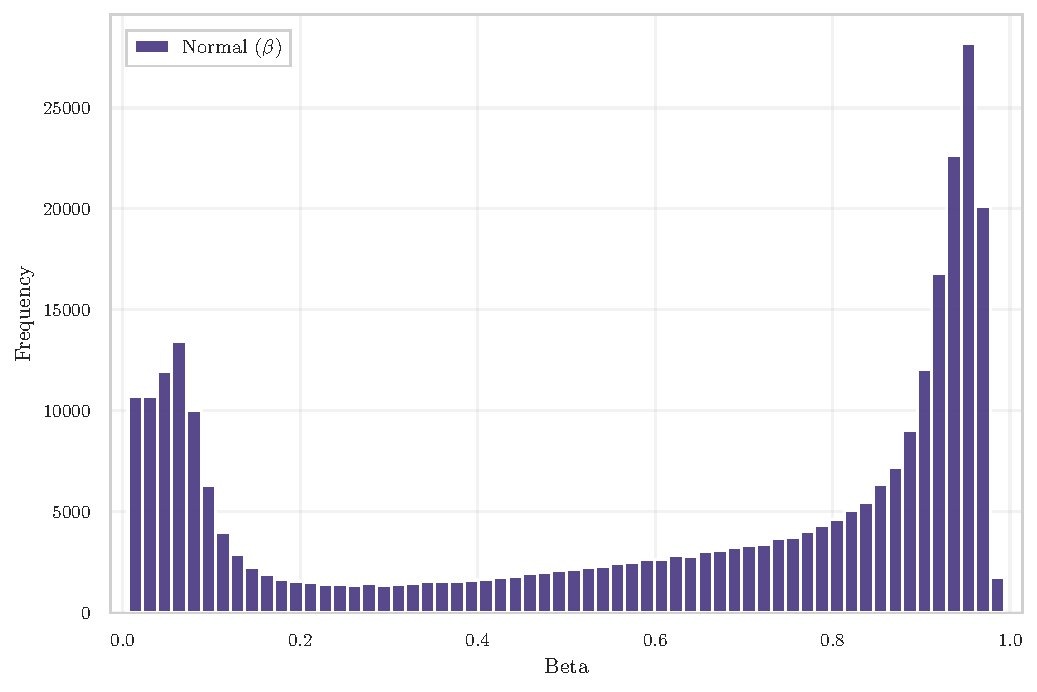
\includegraphics[width=\textwidth]{images/cap4/GSE287331_hist_normal_beta.pdf}
        \caption{Normal ($\beta$)}
    \end{subfigure}
    \begin{subfigure}{0.24\textwidth}
        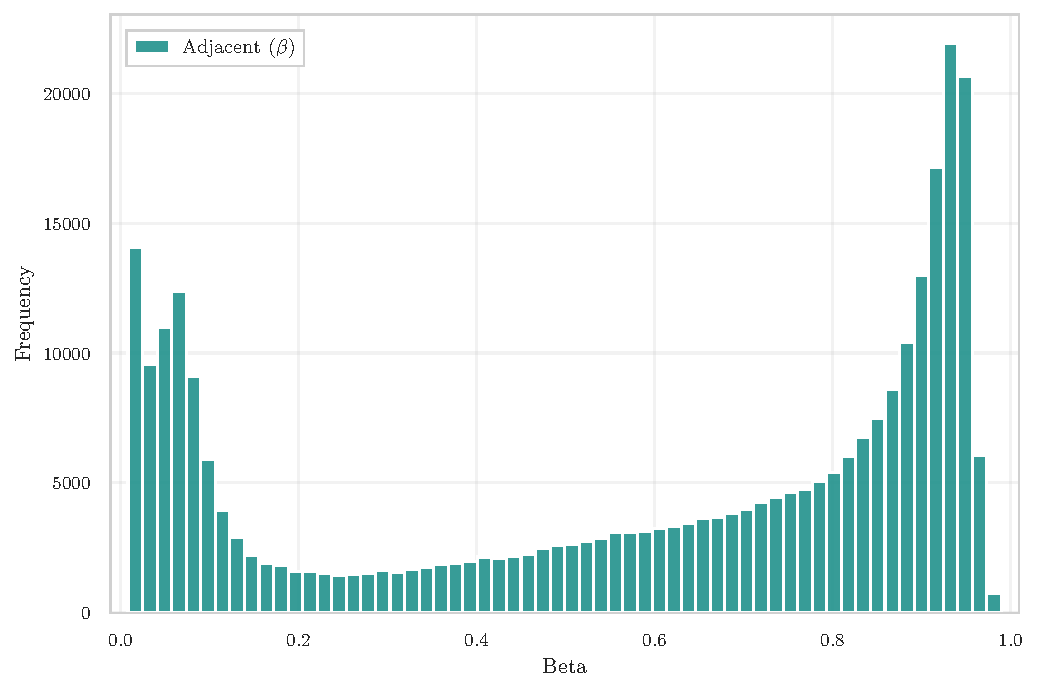
\includegraphics[width=\textwidth]{images/cap4/GSE287331_hist_adjacent_beta.pdf}
        \caption{Adjacent ($\beta$)}
    \end{subfigure}
    \begin{subfigure}{0.24\textwidth}
        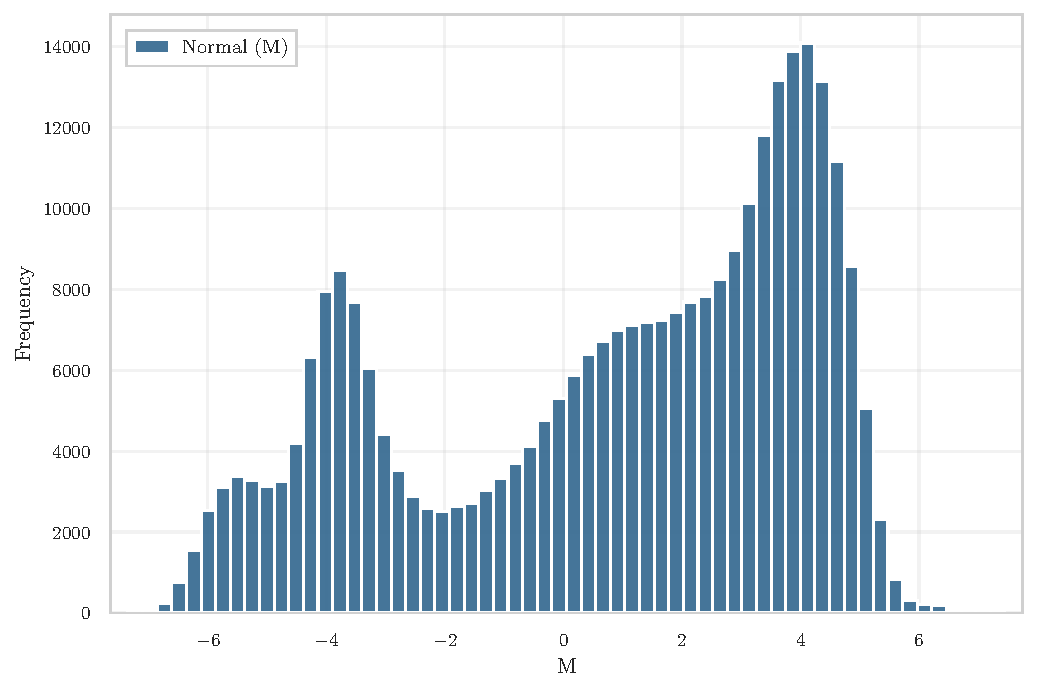
\includegraphics[width=\textwidth]{images/cap4/GSE287331_hist_normal_m.pdf}
        \caption{Normal ($M$)}
    \end{subfigure}
    \begin{subfigure}{0.24\textwidth}
        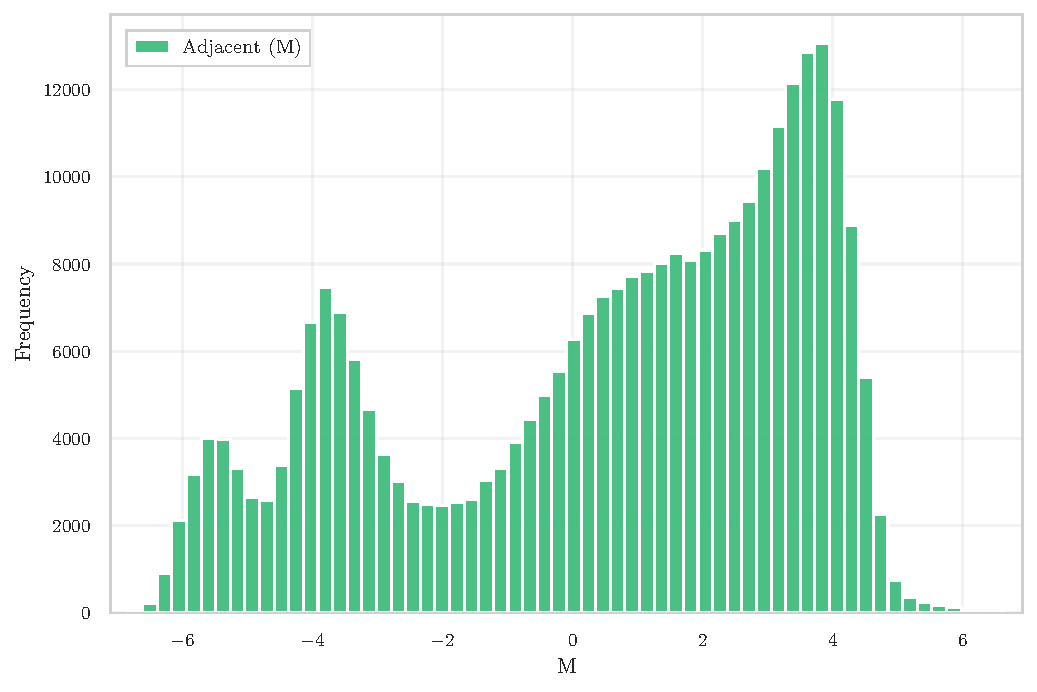
\includegraphics[width=\textwidth]{images/cap4/GSE287331_hist_adjacent_m.pdf}
        \caption{Adjacent ($M$)}
    \end{subfigure}

    \vspace{0.35cm}

    % ---------------- ROW 2: MEAN–SD RELATIONS ----------------
    \begin{subfigure}{0.24\textwidth}
        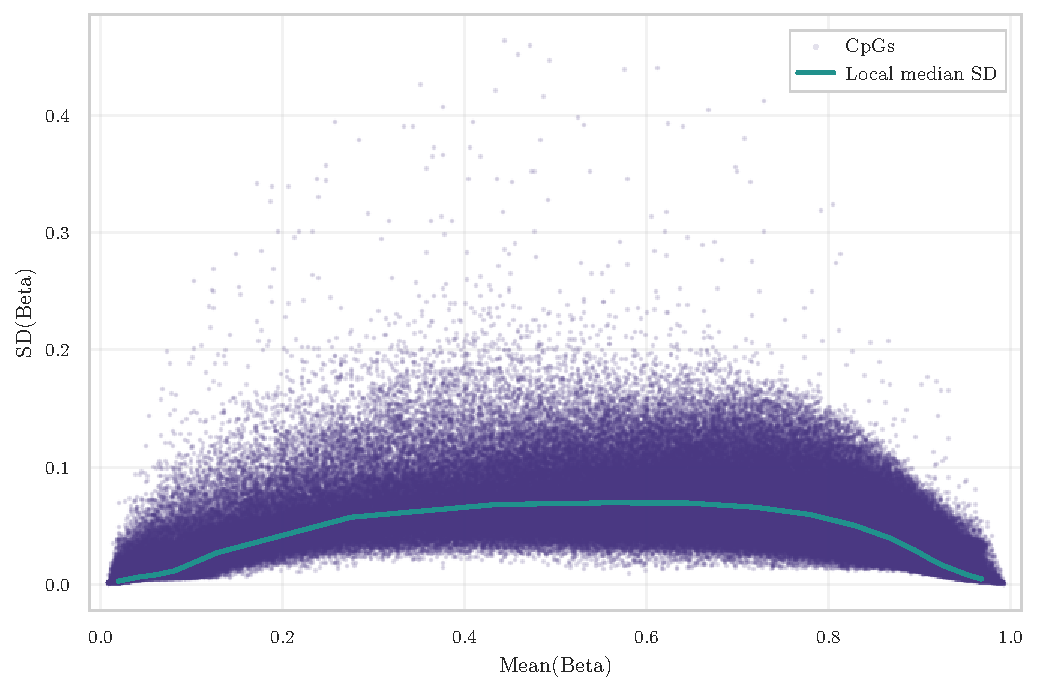
\includegraphics[width=\textwidth]{images/cap4/GSE287331_msd_normal_beta.pdf}
        \caption{Mean--SD (Normal, $\beta$)}
    \end{subfigure}
    \begin{subfigure}{0.24\textwidth}
        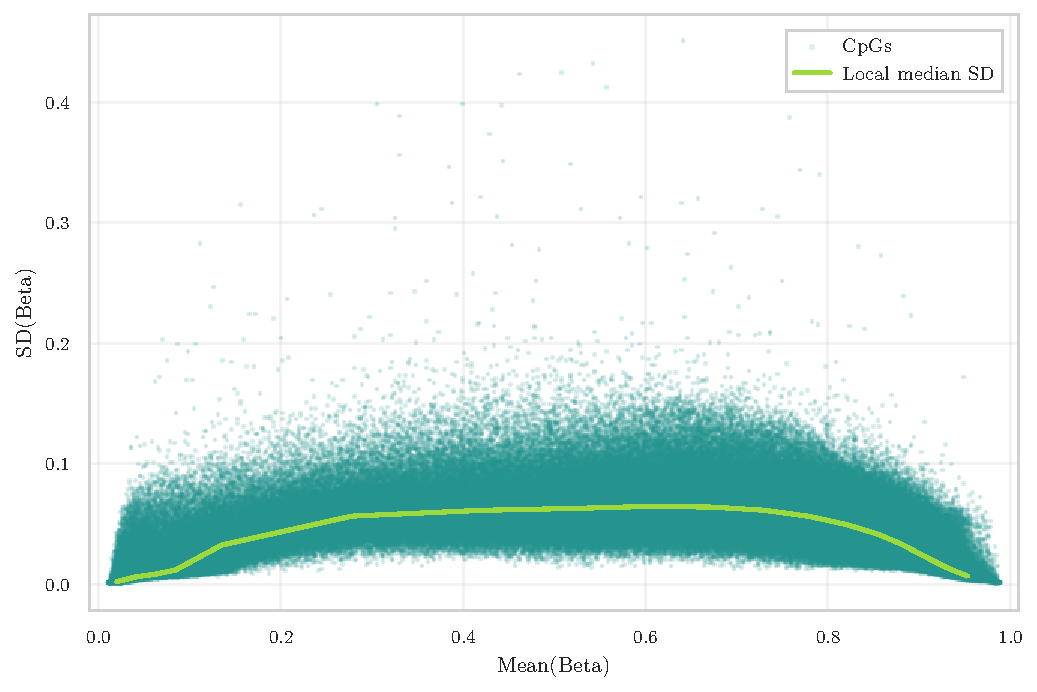
\includegraphics[width=\textwidth]{images/cap4/GSE287331_msd_adjacent_beta.pdf}
        \caption{Mean--SD (Adjacent, $\beta$)}
    \end{subfigure}
    \begin{subfigure}{0.24\textwidth}
        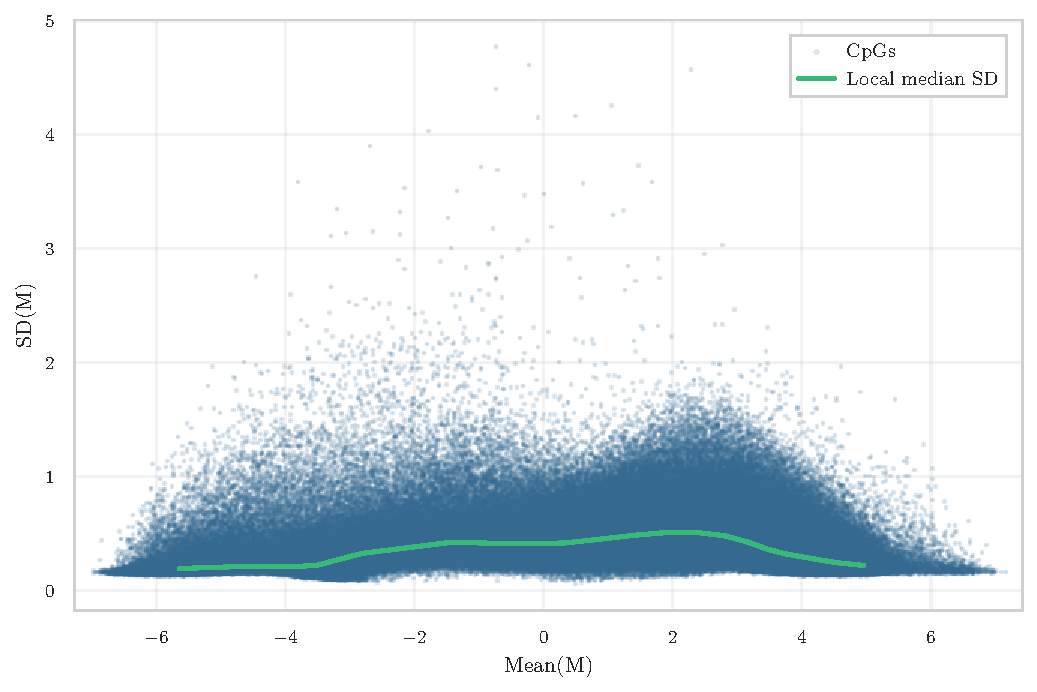
\includegraphics[width=\textwidth]{images/cap4/GSE287331_msd_normal_m.pdf}
        \caption{Mean--SD (Normal, $M$)}
    \end{subfigure}
    \begin{subfigure}{0.24\textwidth}
        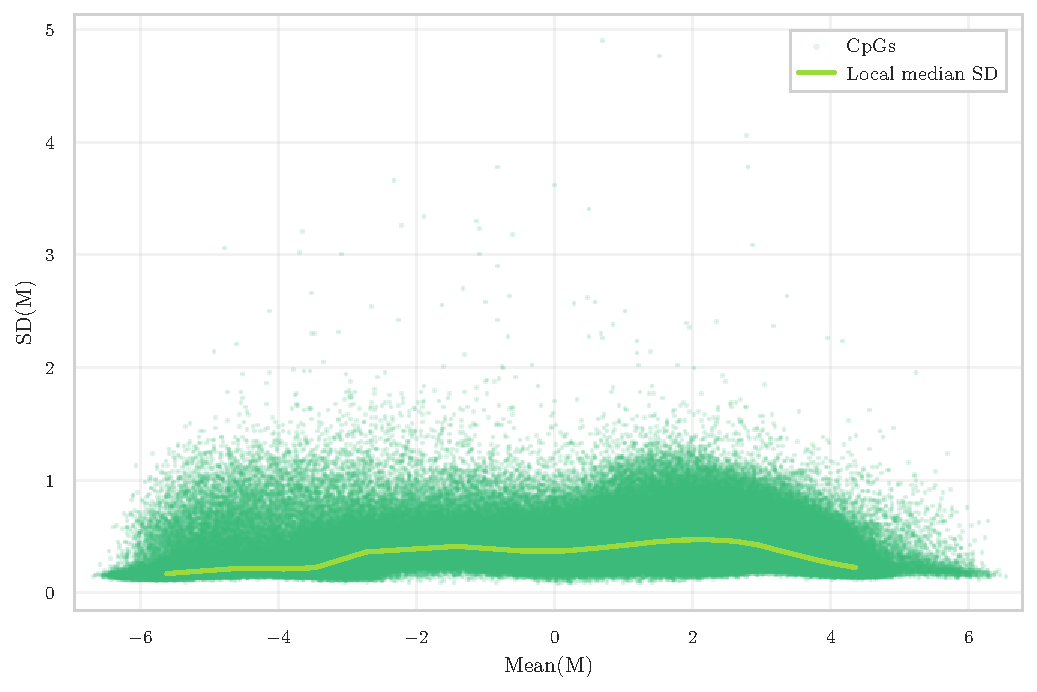
\includegraphics[width=\textwidth]{images/cap4/GSE287331_msd_adjacent_m.pdf}
        \caption{Mean--SD (Adjacent, $M$)}
    \end{subfigure}

    \caption{Distributional comparison of $\beta$ and $M$ in Normal and Adjacent
tissues in GSE287331.}
    \label{fig:gse287331_beta_m_combined}
\end{figure}


Following technical filtering, the $\beta$-value matrix was transformed into
$M$-values using the logit relation defined in Equation~\eqref{eq:mvalue},
in accordance with established recommendations for variance stabilisation
\cite{Du2010, Triche2013Noob, Fortin2017}.
The empirical distributions (Figure~\ref{fig:gse287331_beta_m_combined})
retain the characteristic bounded structure of $\beta$-values; however,
in contrast to GSE69914 and GSE225845, the profiles appear less sharply
bimodal and more broadly dispersed. Both Normal and Adjacent tissues exhibit
reduced concentration at the methylation extremes and a wider intermediate
range, consistent with the greater technical heterogeneity observed in this
cohort.
After transformation, the corresponding $M$-value distributions become more
symmetric, as expected under the logit mapping, yet remain visibly broader
than in the other datasets. The mean--SD relationships confirm that while
variance stabilisation is achieved, dispersion remains comparatively elevated
across the full methylation range. This behaviour is coherent with the
stronger preprocessing burden documented in earlier steps and reflects the
intrinsic variability of the released matrix.


% ============================================================

\begin{figure}[t]
\centering
\begin{subfigure}[t]{0.48\textwidth}
    \centering
    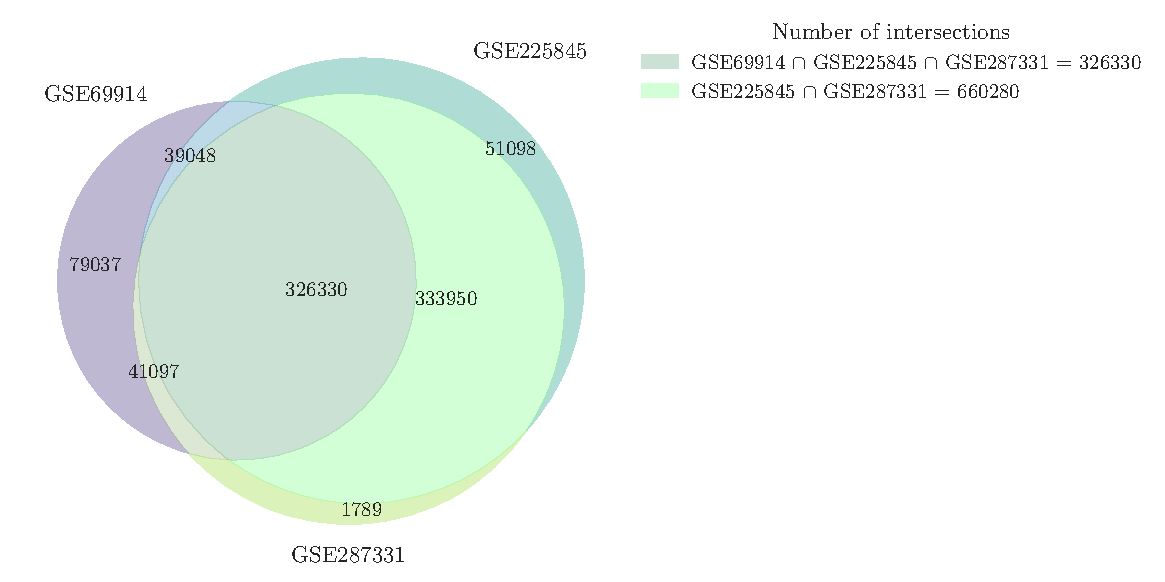
\includegraphics[width=\textwidth]{images/cap4/venn_cpg_overlap_pre_preprocessing.pdf}
    \caption{CpG overlap before preprocessing.}
    \label{fig:venn-pre}
\end{subfigure}
\hfill
\begin{subfigure}[t]{0.48\textwidth}
    \centering
    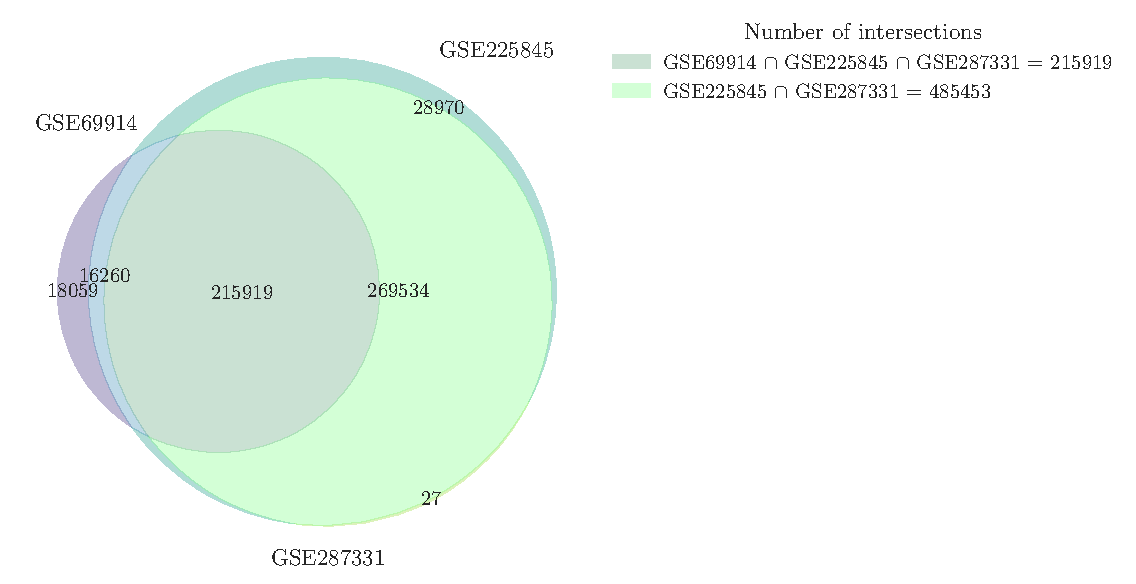
\includegraphics[width=\textwidth]{images/cap4/venn_cpg_overlap_post_preprocessing.pdf}
    \caption{CpG overlap after preprocessing.}
    \label{fig:venn-post}
\end{subfigure}
\caption{CpG overlap across datasets before and after preprocessing.}
\label{fig:venn-comparison}
\end{figure}

\section{Inter-Dataset Consistency After Preprocessing}
\label{sec:inter_preprocessing}

After completing the intra-dataset preprocessing for each cohort, a concise
inter-dataset analysis is performed to summarise the effects of the pipeline
and to motivate the subsequent feature selection step.

\paragraph{Consistency of the Preprocessing Framework}
All three datasets underwent a harmonised preprocessing workflow, including
initial integrity checks, literature-based technical filtering, manifest-driven
probe validation, removal of sex-chromosome loci, and transformation from
$\beta$-values to M-values. While specific implementation details differ slightly
depending on platform characteristics and data quality, the conceptual structure
of the pipeline is consistent across datasets.
Table~\ref{tab:preprocessing-summary} reports, for each dataset, the
dimensionality of the methylation matrix before and after preprocessing. Despite
substantial differences in initial platform coverage (450K vs.\ EPIC), technical
filtering consistently removes a large fraction of probes, yielding cleaner and
more reliable feature spaces.

\paragraph{CpG overlap across datasets}
CpG overlap was evaluated both before and after preprocessing to characterise
the relationship between cohorts. Prior to filtering
(Figure~\ref{fig:venn-pre}), the intersection is dominated by probes shared
between the two EPIC datasets, with a smaller but substantial core common to
all three cohorts, reflecting platform design constraints and baseline
annotation differences. After the complete preprocessing pipeline
(Figure~\ref{fig:venn-post}), the total number of CpGs is markedly reduced,
yet a large shared core is preserved: the three-way intersection comprises
215{,}919 CpGs, representing a stable autosomal backbone consistently
retained across platforms after technical filtering.


\begin{table}[t]
\centering
\caption{CpG dimensionality before and after preprocessing.}
\label{tab:preprocessing-summary}
\scriptsize
\begin{tabular}{l c c c}
\toprule
Dataset & Platform & CpGs \textit{before} & CpGs \textit{after} \\
\midrule
GSE69914  & 450K & 485{,}512 & 251{,}483 \\
GSE225845 & EPIC & 750{,}426 & 530{,}683 \\
GSE287331 & EPIC & 866{,}554 & 486{,}725 \\
\bottomrule
\end{tabular}
\end{table}

\section{Post-Preprocessing Feature Space and Dimensionality Implications}
\label{sec:postproc_rationale}

The preprocessing pipeline developed in this chapter has systematically
addressed the three main classes of technical confounders identified in
Chapter~\ref{sec:data_preparation_exploration}: probe-design bias,
unreliable probe sets, and statistical scale distortion. The resulting
matrices are technically clean, fully observed, and expressed on a
variance-stabilised $M$-value scale suitable for inferential modelling.
Across all three cohorts, the three-way CpG intersection comprises
215{,}919 autosomal loci retained after platform-aware filtering,
constituting a stable and harmonised feature backbone for cross-dataset
analyses.
Yet the preprocessing outcome also sharpens the central analytical
challenge. The post-processed datasets remain extremely high-dimensional
--- 251{,}483 CpGs in GSE69914, 530{,}683 in GSE225845, and 486{,}725
in GSE287331 --- and the exploratory analyses of
Chapter~\ref{sec:data_preparation_exploration} established that the
Normal--Adjacent signal is focal and low-amplitude, with mean
$|\Delta\beta|$ ranging from 0.009 to 0.031 across cohorts. In this
regime, the overwhelming majority of retained CpGs carry no
discriminative information for the contrast of interest: including them
in downstream modelling would dilute the signal, inflate variance
estimates, and compromise both interpretability and generalisation.
The limiting factor is therefore no longer data quality but
\emph{signal localisation}: identifying the restricted subset of CpG
loci that capture biologically meaningful Normal--Adjacent variation,
consistently across cohorts and independently of platform-specific
noise. This requires a principled feature selection strategy that is
sensitive to the subtle, focal nature of the epigenetic drift documented
here, robust to the cohort-level heterogeneity observed in the
inter-dataset comparisons, and compatible with the homoscedastic
$M$-value representation adopted for modelling.

Chapter~\ref{chap:feature_selection} addresses this challenge directly,
developing and evaluating feature selection methodologies applied
separately within each dataset-specific CpG space. In order to preserve
the full informational richness of the EPIC platforms, feature selection
is not restricted to the three-way CpG intersection but is performed on
the complete post-processed feature set of each cohort, thereby avoiding
artificial dimensional truncation driven by the lower coverage of the
450K array.
